\section{Specific System Description}\label{sec_SpecDesc}
This section first presents the problem description, giving a high-level view 
of the problem to solve (\ref{Sec_pd}), some terminology and definitions to 
clarify models, data, and requirements (Section~\ref{sec_terms}), and goals 
that a solution must achieve (Section~\ref{sec_goals}). It then describes 
characteristics of a potential solution, including Assumptions 
(Section~\ref{sec_assumptions}), Theoretical Models 
(Section~\ref{sec_theoretical}), General and Data Definitions 
(Sections~\ref{sec_gendef} and~\ref{sec_datadef}), Data Types 
(Section~\ref{sec_typedefs}), and the Instance Models derived from these 
(Section~\ref{sec_instance}). This is followed by Constraints 
(Section~\ref{sec_DataConstraints}) and Properties of a Correct Solution 
(Section~\ref{sec_CorrectSolution}).

One section---Conceptual Models (Section~\ref{sec_conceptual})---has been added 
to the solution characteristics that is not in the SRS template in 
\cite{SmithAndLai2005} and \cite{SmithEtAl2007}. It is useful for maintaining a 
direct connection to the affective research behind the Theoretical and Instance 
Models. The Theoretical Models also differ from those in the template, focusing 
on rewriting descriptions in the Conceptual Models with more precise natural 
language. This shows what interpretation of the Conceptual Models that lead to 
their mathematical representations in the Data Types and Instance Models.

\subsection{Problem Description} \label{Sec_pd}
The purpose of \progname{} is to generate an emotion state for an entity, as 
well as store and update said emotion state with generated or given data. It 
must be done to afford users the most control over when and how \progname{} 
generates emotion with only a layperson's understanding of emotion and emotion 
processes.

\subsubsection{Terminology and  Definitions}\label{sec_terms}
The Conceptual Models (Section~\ref{sec_conceptual}) contain many definitions 
necessary for reducing ambiguity and making it easier to understand models and 
requirements. These are additional terms that do not appear in the Conceptual 
Models, but are still useful for the same reasons. \\

\noindent\textbf{Affect}: Any type of affective experience that has a
changeable, short-term state originating from the body and impacting the
mind in some way~\citep{barrett2009affect, oxfordAffect}. A general
affective state is generally identified as weaker than an emotion state. \\

\noindent\textbf{Affective Science}: The interdisciplinary study of affective 
phenomena, related processes, and its influencing 
factors~\citep[p.~xiii]{davidson2003handbook}. \\

\noindent\textbf{Appraisal Theories (Perspective)}: These theories shift the 
evaluation of the environment from its objective qualities to its relation to 
an individual's well-being~\citep[p.~86]{smith2000consequences}. They mainly 
focus on the link between cognitive processing and emotion 
elicitation~\citep[p.~354]{broekens2021emotion}. \\

\noindent\textbf{Arousal}: A short-term state of excitement or energy
expenditure~\citep{oxfordArousal}. \\

\noindent\textbf{Cognition}: ``All forms of knowing and awareness, such as
perceiving, conceiving, remembering, reasoning, judging, imagining, and problem
solving''~\citep{cognitiondef}. \\

\noindent\textbf{Core Affect}: Based on affect, ``...a state of pleasure or
displeasure with some degree of arousal''~\citep[p.~170]{barrett2009affect}.
See also \textit{Affect}. \\

\noindent\textbf{Dimensional Theories (Perspective)}: These theories can more 
easily distinguish between different emotions (\citepg{scherer2010emotion}{12}; 
\citepg{smith1985patterns}{813}) using a small number of continuous dimensions. 
They view emotion as an individual's interpretation of their current ``core 
affect''~\citep[p.~353]{broekens2021emotion} (i.e. elementary affective 
feelings). While any point in dimensional space is part of ``core 
affect''~\citep[p.~97]{lisetti2015and}, it is possible for individuals to 
verbally label points representing their subjective feeling of an 
emotion~\citep[p.~12]{scherer2010emotion}. This creates an effect of 
``plotting'' emotion categories (e.g. discrete theories) as points in the 
space. \\

\noindent\textbf{Discrete Theories (Perspective)}: These theories propose that 
innate, hard-wired circuits or programs elicit emotions 
(\citepg{ortony2021all}{41}; \citepg{scherer2021towards}{280}). One of the core 
features of these theories is the definition of distinct
emotion categories or types, like \textit{Joy} and \textit{Anger}, that are
recognizable by a set of observable features (e.g. facial expression, typical
behaviours). This ``...fits with the way we talk about emotion every
day...people automatically and effortlessly perceive emotion in themselves and
others...''~\citep[p.~47--48]{barrett2006emotions}. \\

\noindent\textbf{Emotion Expression}: An affective computing task where a CME
changes an entity's ``observable'' behaviour (e.g. facial expressions,
gestures, or movements) given an emotion state (\citepg{scherer2010emotion}{4};
\citepg{fathalla2020emotional}{2}). \\

\noindent\textbf{Emotion Generation}: An affective computing task where a CME
produces an emotion state given the current program and environment state
(\citepg{scherer2010emotion}{4}; \citepg{fathalla2020emotional}{2}). \\

\noindent\textbf{Emotion Kind}: Names given to discrete categories/types of
emotion (e.g. \textit{Joy}, \textit{Sadness}). \\

\noindent\textbf{Emotion State}: The set of values for each possible emotion
kind. \\

\noindent\textbf{Entity}: Any discrete, identifiable, and separate object that
is significant in and of themselves. \\

\noindent\textbf{``Fast, Primary Emotions''}: Hard-wired and potentially 
inaccurate responses to innate knowledge elicited by fundamental mechanisms 
(e.g. instinctual fear of pain)~\citep[p.~60--70]{picard1997affective}. \\

\noindent\textbf{Feeling}: Conscious mental representations and interpretations
of an emotional response, and follow emotions evolutionarily and experientially
(\citepg{oxfordFeelings}{184}; \citepg{scherer2000psychological}{139}).
Feelings are ill-defined from a modelling perspective, and rarely, if ever,
appear computationally. They are also, allegedly, unnecessary for understanding
emotional behaviours~\citep{fellous2004human}. \\

\noindent\textbf{Game World}: An imaginary universe in which game events  take
place~\citep{adams2014fundamentals}. They are often two or three dimensional
spaces containing characters and objects. \\

\noindent\textbf{Global Adaptational Problem}: In PES, a survival-related issue
that emotion-based behaviours evolved to address and are found in some form at
all evolutionary levels~\citep{robert1980emotion}. \\

\noindent\textbf{Gustatory}: Concerned with tasting or the sense of taste. In
CTE, this is associated with the mental process of withdrawing from toxins and
potentially infectious agents~\citep[p.~57]{oatley1992best}. In this way, it
could also be a prototype for other withdrawal-based emotions (e.g.
\textit{Hatred}, \textit{Contempt}). \\

\noindent\textbf{``Model of Self''}: In CTE, a cognitive representation of the
individual's own goals, abilities, habits, and bodies, chiefly in relation with
others~\citep[p.~195]{oatley1992best}. \\

\noindent\textbf{Mood}: Enduring, less intense, and more diffuse states than
emotions~\citep{oxfordMood}. Their presence is typically unclear to the
experiencing individual and often have a more prolonged influence on an
individual’s cognition and behaviours. \\

\noindent\textbf{Non-propositional Meaning}: In relation to communication,
signals with no symbolic structure or literal meaning of significance within a
system~\citep[p.~32]{oatley1987towards}. \\

\noindent\textbf{Personality}: Permanent or difficult to change variables that
impact affective processes~\citep{oxfordPersonality}. \\

\noindent\textbf{Propositional Meaning}: In relation to communication, signals
having a symbolic structure with a literal meaning of significance to a
system~\citep[p.~32]{oatley1987towards}. \\

\noindent\textbf{Self-Preservational}: In relation to self-preservation,
especially regarded as a basic instinct in human beings and animals, the
protection of oneself from harm or death. \\

\noindent\textbf{``Slow, Secondary Emotions''}: Sometimes called 
``cognitively-generated emotions'', these require some level of reasoning to 
elicit (e.g. learned fear of public 
speaking)~\citep[p.~60--70]{picard1997affective}. \\

\noindent\textbf{Valence}: Describes the positive or negative character of
emotions, their response components, and emotion-eliciting
stimuli~\cite{oxfordValence}. In affective science, it often appears as a
dimensional variable with positive and negative poles. Assigning valence to
an emotion depends on its context (e.g. behavioural tendencies vs. social
interactions).

\subsubsection{Physical System Description}
\progname{} does not interact with a physical system, and is not concerned with
the physical hardware that the run-time environment and its components run on
or how it generates data.

\subsubsection{Goal Statements}\label{sec_goals}
Given an entity that is associated with at least one instance of \progname{},
the entity's goals, a world state, an event that changes or could change that
world state, and optional world and/or entity knowledge, \progname{}'s goals
are:
\begin{itemize}

    \item[GS\refstepcounter{goalnum}\thegoalnum \label{G_EmotionGeneration}]
    Determining what emotion type and intensity is elicited by a change in game
    world state.

    \item[GS\refstepcounter{goalnum}\thegoalnum \label{G_EmotionDecay}]
    Determining what intensity each emotion type has when decaying emotion.

    \item[GS\refstepcounter{goalnum}\thegoalnum \label{G_UpdateEmotionState}]
    Updating stored emotion values.

    \item[GS\refstepcounter{goalnum}\thegoalnum \label{G_QueryEmotionState}]
    Allowing queries about stored emotion values.

\end{itemize}

The goal statements only describe \progname{}'s \textit{tasks}. \progname{}
also requires goals (i.e. high-level requirements) describing its target
\textit{properties} to guide the selection of its underlying emotion theories
(Section~\ref{sec_theories}). This process is needed to define the Assumptions
(Section~\ref{sec_assumptions}) and Conceptual Models
(Section~\ref{sec_conceptual}). The high-level requirements directly
incorporate some of the needs of video game designers/developers
(Section~\ref{sec:doc_stakeholder}) to improve the probability of \progname{}'s
acceptance, which the SRS incorporates in the nonfunctional requirements
(Section~\ref{sec_ReqsNF}).

The \textit{flexibility} goals are about making \progname{} adaptable so that
it can meet game designer needs~\citep[p.~30]{reilly1996believable}. The aim is
for \progname{} to be applicable to a range of game designs while avoiding
making decisions for the game developer.
\begin{enumerate}[label=RF\arabic*]
    \item\label{flexArch} Independence from an agent architecture so that
    designers can choose how to integrate \progname{} into their game
    (\citepg{loyall1997believable}{25--26};
    \citepg{rodriguez2015computational}{443};
    \citepg{broekens2016emotional}{218})

    \item\label{flexTasks} Allowing the game designer to choose which of
    \progname{}'s tasks to use, as well as when and how to use
    them (\citepg{mascarenhas2022fatima}{8:13};
    \citepg{guimaraes2022fatima}{20})

    \item\label{flexCustom} Allowing the customization or redefinition of
    \progname{}'s pre-existing configuration parameters
    (\citepg{reilly1996believable}{30}; \citepg{guimaraes2022fatima}{20})
    such as the definition of time and emotion decay rates

    \item\label{flexNew} Allowing designers to integrate new components
    into \progname{} that influence or are influenced by emotion
    (\citepg{rodriguez2015computational}{450};
    \citepg{castellanos2019mechanism}{353}), such as mood, personality,
    motivations, culture, gender, and physical state

    \item\label{flexEm} Allowing designers to choose which kinds of emotion
    \progname{} produces (i.e. which emotions an NPC can
    have)~\citep[p.~331]{hudlicka2014computational}, (e.g. \textit{Anger},
    \textit{Joy})

    \item\label{flexOut} Allowing designers to specify how to use
    \progname{}'s outputs~\citep[p.~86]{loyall1997believable}

    \item\label{flexComplex} Allow designers to use \progname{} on
    different levels of NPC
    complexity~\citep[p.~220]{broekens2016emotional}, e.g. a
    \textit{Pac-man} ghost~\citep{pacman} and a \textit{Skyrim}
    citizen~\citep{skyrim} will not have the same emotional requirements

    \item\label{flexScale} Being efficient and scalable to minimize
    \progname{}'s impact on overall game performance
    \citep[p.~42]{popescu2014gamygdala}
\end{enumerate}

The \textit{ease-of-use} goals concern the usability of \progname{} and showing
how it supports game development. These aim to make \progname{} more
user-friendly and minimize maintenance to increase its chances of adoption by
game developers.
\begin{enumerate}[label=RE\arabic*]
    \item\label{easeHide} Hiding the complexity of emotion generation so
    that game designers do not have to be knowledgeable in emotion
    psychology to use \progname{} (\citepg{reilly1996believable}{28};
    \citepg{broekens2016emotional}{220}; \citepg{guimaraes2022fatima}{5})

    \item\label{easeAPI} Providing a clear and understandable Application
    Programming Interface (API) or similar that shows how to use the
    different aspects of \progname{}~\citep[p.~218]{broekens2016emotional}

    \item\label{easeAuthor} Minimizing authorial burden as game developers
    add NPCs to their game~\citep[p.~5]{guimaraes2022fatima}

    \item\label{easeTrace} Allowing \progname{}'s outputs to be traceable
    and understandable (\citepg{loyall1997believable}{86};
    \citepg{guimaraes2022fatima}{5, 19--20})---critical for testing---by
    providing ways to view the range, intensity, and causes of emotion per
    NPC, per NPC group, and per game world
    area~\citep[p.~219--220]{broekens2016emotional}

    \item\label{easeAuto} Allowing developers the option to automate the
    storing and decaying of \progname{}'s internal emotion
    state~\citep[p.~86]{loyall1997believable}

    \item\label{easePX} Showing that \progname{} improves the player
    experience, since a sub-par design could be a detriment to the overall
    game and would not be of use to game development

    \item\label{easeNovel} Providing examples as to how \progname{} can
    create novel game experiences~\citep[p.~221]{broekens2016emotional}
\end{enumerate}

The flexibility and ease-of-use goals also imply that \progname{} \textit{must
not} depend on a particular entity embodiment or implementation because this
limits the types of entities that it could support (related to \ref{flexArch},
\ref{flexComplex}), and it \textit{must} support the generation of
\textit{fast, primary emotions} and \textit{slow, secondary
emotions}~\citep[p.~60--70]{picard1997affective} (related to \ref{flexComplex}).

\newpage

\subsection{Solution Characteristics Specification}\label{Sec_scs}

This section expresses \progname{}'s solution characteristics in mathematical
form via Data Types (Section \ref{sec_typedefs}) and Instance Models
(Section~\ref{sec_instance}), as well as underlying Assumptions
(Section~\ref{sec_assumptions}), Data Constraints
(Section~\ref{sec_DataConstraints}) and additional properties necessary for
\progname{} to be correct (Section~\ref{sec_CorrectSolution}). These components
are refinements of Theoretical Models (Section~\ref{sec_theoretical}), which
are in turn refinements of Conceptual Models (Section~\ref{sec_conceptual}).
They are necessary for understanding the Data Types and Instance Models so that
they can be verified.

\subsubsection{Emotion Theories and Models}\label{sec_theories}
All potential \progname{} solutions must be based on emotion theories and data
to improve its \textit{psychologically validity}, which is necessary for its
behaviours to be \textit{plausible}~\citep[p.~216--217]{broekens2016emotional}.
The theories that \progname{} uses must align with its overall design goals.

\progname{}'s theories are Oatley \& Johnson-Laird's Communicative Theory of
Emotion (CTE), Plutchik's Psycho-Evolutionary Synthesis (PES), and Mehrabian's
Pleasure-Arousal-Dominance Space (PAD). These were chosen from a pool of
potential candidates (Table~\ref{tab:theories}) based on their ability to
satisfy the \textit{flexibility} and \textit{ease-of-use} high-level
requirements (Section~\ref{sec_systemConstraints}). Note that these
requirements are theory-agnostic, so any emotion theory that supports them is a
reasonable choice.

The selection process follows these general steps:
\begin{enumerate}
    \item Scoping the high-level requirements as needed
    \item Scoring each candidate theory
    \item Choosing theories based on their scores
\end{enumerate}

\paragraph{Scoping}
The analysis separates \textit{Providing a clear and understandable API}
(\ref{easeAPI}) into two---Input and Output---to get a better feel for each
theory's usefulness. This is an acknowledgement that some theories are better
for emotion expression, such as Ekman \& Friesen.

The requirement for \textit{Allowing the Integration of New Components}
(\ref{flexNew}) is broad and should be scoped for the initial design of
\progname{}. New \progname{} components could be non-affective (e.g. attention)
and affective (e.g. personality) in nature. Integrating non-affective
components should be theory-agnostic, as they are part of separate components
of mind~\citep{cognitiondef}. From a software engineering perspective, one
could view the mind as a system with distinct, interacting subsystems. Modular
interfaces that control interactions between \progname{}---as the affective
subsystem---and components from other subsystems would support this concept,
while also maintaining \progname{}'s requirements for \textit{Independence from
an Agent Architecture} (\ref{flexArch}) and \textit{Allowing Developers to
Specify How to Use Outputs} (\ref{flexOut}). Integrating other affective
components would depend on \progname{} and its foundational theories. One would
be limited to only those components that can be represented in terms of the
emotions or other types of affect that have been connected to them.

This requirements analysis focuses on three other types of affect: core affect,
mood, and personality. Of these, it prioritizes personality because it is
necessary for creating the consistent and coherent agent behaviours that
influence believability (\citepg{reilly1996believable}{26};
\citepg{loyall1997believable}{19}; \citepg{ortony2002making}{203}).

Finally, the \textit{Minimizing authorial burden} requirement
(\ref{easeAuthor}) is excluded from the analysis. This is due to its focus on
helping game developers manage the creation of an increasing NPC population,
rather than the functionality of \progname{} itself.

\begin{table}[!tbh]
    \renewcommand{\arraystretch}{1.2}
    \centering
    \caption{Theories Analysed}
    \label{tab:theories}
    \begin{tabular}{P{0.2\columnwidth}P{0.65\columnwidth}}
        \toprule
        \textbf{Perspective} & \textbf{Theories} \\
        \midrule

        \rowcolor[gray]{0.9}Discrete & Ekman \& Friesen (Ek.), Izard (Iz.),
        Plutchik (Plu.) \\

        Dimensional & Valence-Arousal (V-A), PAD Space (PAD) \\

        \rowcolor[gray]{0.9}Appraisal & Frijda (Frj.), Lazarus (Laz.), Scherer
        (Sch.), Roseman (Ros.), Ortony, Clore, and Collins (OCC), Smith \&
        Kirby (S \& K), Oatley \& Johnson-Laird (O \& JL) \\

        \bottomrule
    \end{tabular}
\end{table}

\paragraph{Scoring} Each theory has a set of notes made during their
examination, guided by individual high-level requirements. After reviewing the
notes, each theory is assigned a \textit{score} describing its relative
``suitability'' for that requirement (Table~\ref{tab:scoring}). This step is
somewhat subjective because a judgement is made without true objective measures
or methods. The notes are in Appendix~\ref{chapter:reqsTheoryNotes}.

\progname{}'s high-level requirements are divided into two sets:
\textit{system-level}, which applies to \progname{} as a whole
(Tables~\ref{tab:theory-req-sys-summary-flexibility} and
\ref{tab:theory-req-sys-summary-easeofuse}), and \textit{component-level} for
requirements that only apply to specific pieces of \progname{}
(Tables~\ref{tab:theory-req-comp-summary-flexibility} and
\ref{tab:theory-req-comp-summary-easeofuse}). Only appraisal theories are
assigned categories for component-level requirements because they concern
process-related elements that discrete and dimensional theories do not address.
Each theory has unique elements, which might make it better or worse suited for
a particular requirement. These are noted in the analysis. However, is not
unusual for theories from the same perspective to satisfy a requirement equally
well. In these cases, the theories are treated as a collective unit when
examining the requirement.
Tables~\ref{tab:theory-req-sys-summary-flexibility},
\ref{tab:theory-req-sys-summary-easeofuse},
\ref{tab:theory-req-comp-summary-flexibility}, and
\ref{tab:theory-req-comp-summary-easeofuse} summarize the scores for each
theory and requirement.

\begin{table}[!h]
    \renewcommand{\arraystretch}{1.2}
    \centering
    \caption{Summary of Scoring Categories}
    \label{tab:scoring}
    \begin{tabular}{ccP{0.65\columnwidth}}
        \toprule
        \textbf{Score Category} & \textbf{Symbol} & \textbf{Definition} \\

        \midrule

        \rowcolor[gray]{0.9}\textit{Strong} & \strong & The theory
        appears to satisfy the requirement in a clear, understandable way and
        is likely to aid in \progname{}'s usability
        \\

        \textit{Good} & \good & The theory appears to satisfy the requirement
        and is somewhat defined \\

        \rowcolor[gray]{0.9}\textit{Weak} & \weak & The theory
        describes ways that \textit{could} satisfy the requirement, but it is
        not fully defined or could make \progname{} harder to use \\

        \textit{Disqualified} & \disqualified & The theory does not seem likely
        to be able to satisfy this requirement, or it violates other
        requirements when it can (including psychological validity) \\

        \bottomrule

    \end{tabular}
\end{table}

\begin{table}[!tbh]
    \renewcommand{\arraystretch}{1.2}
    \centering
    \caption[Support for System-Level Flexibility High-Level
    Requirements]{Support for System-Level \textbf{Flexibility} High-Level
        Requirements}
    \label{tab:theory-req-sys-summary-flexibility}
    \footnotesize
    \begin{threeparttable}
        \begin{tabular}{@{}cP{0.13\linewidth}cccccccccccc@{}}

            \toprule
            \multicolumn{2}{c}{} & \hd{\textbf{Ek.}} &
            \hd{\textbf{Iz.}} & \hd{\textbf{Plu.}} & \hd{\textbf{V-A}}
            & \hd{\textbf{PAD}} & \hd{\textbf{Frj.}} &
            \hd{\textbf{Laz.}\textsuperscript{\footnotesize\textpmhg{\Hi}}} &
            \hd{\textbf{Sch.}} & \hd{\textbf{Ros.}} &
            \hd{\textbf{OCC}} & \hd{\textbf{S \& K}} & \hd{\textbf{O \&
                    JL}} \\
            \midrule

            \rowcolor[gray]{0.9}\ref{flexArch} & \textit{Independence
                from an Agent Architecture} & {\normalsize\good} &
            {\normalsize\good} & {\normalsize\good} & {\normalsize\good} &
            {\normalsize\good} & {\normalsize\strong} & {\normalsize\good} &
            \disqualified & {\normalsize\good} & {\normalsize\strong} &
            {\normalsize\strong} & {\normalsize\strong} \\

            \ref{flexNew} & \textit{Allowing the Integration of
                Components}{\large\textpmhg{\Hl}} & {\normalsize\weak} &
            {\normalsize\weak}\textsuperscript{\normalsize\Moon} &
            {\normalsize\good}\textsuperscript{\normalsize\Moon} &
            {\normalsize\strong}\textsuperscript{\large\Jupiter} &
            {\normalsize\strong}\textsuperscript{\large\Jupiter} &
            {\normalsize\strong} & {\normalsize\weak} & {\normalsize\weak} &
            {\normalsize\weak} & {\normalsize\strong} & {\normalsize\weak} &
            {\normalsize\strong} \\

            \rowcolor[gray]{0.9}\ref{flexEm} & \textit{Choosing NPC
                Emotions} & {\normalsize\weak} & \disqualified &
            {\normalsize\strong} & {\normalsize\weak} & {\normalsize\good} &
            {\normalsize\weak} & {\normalsize\weak} & {\normalsize\good} &
            {\normalsize\good} & {\normalsize\good} & {\normalsize\weak} &
            {\normalsize\strong} \\

            \ref{flexOut} & \textit{Allowing Developers to Specify How to Use
                CME Outputs} & {\normalsize\good} & {\normalsize\good} &
            {\normalsize\good} & {\normalsize\strong} & {\normalsize\strong} &
            {\normalsize\strong} & {\normalsize\strong} & {\normalsize\strong} &
            {\normalsize\strong} & {\normalsize\strong} & {\normalsize\strong}
            & {\normalsize\strong} \\

            \rowcolor[gray]{0.9}\ref{flexComplex} & \textit{Ability to
                Operate on Different Levels of NPC Complexity} &
                {\normalsize\good}
            & {\normalsize\good} & {\normalsize\good} & {\normalsize\weak} &
            {\normalsize\weak} & {\normalsize\weak} & {\normalsize\strong} &
            {\normalsize\strong} & {\normalsize\good} & {\normalsize\good} &
            {\normalsize\strong} & {\normalsize\good} \\

            \ref{flexScale} & \textit{Be Efficient and Scalable} &
            {\normalsize\good} & {\normalsize\good} & {\normalsize\good} &
            {\normalsize\weak} & {\normalsize\weak} &
            {\normalsize\good}\textsuperscript{\large\Pluto} &
            {\normalsize\strong} & {\normalsize\good} & {\normalsize\weak} &
            {\normalsize\good} & {\normalsize\strong} & {\normalsize\strong} \\

            \hline\bottomrule
        \end{tabular}
        \begin{tablenotes}

            \footnotesize
            \vspace*{2mm}

            \item \textit{See Table~\ref{tab:scoring} for score category
                descriptions.}

            \item {\small\textpmhg{\Hi}} \textit{Excludes the
                \textit{Coping Process} because it is part of action
                generation.}

            \item {\Large\textpmhg{\Hl}} \textit{Strictly focusing on
                core affect, mood, and personality.}

            \item {\normalsize\Moon} \textit{Natively supports integration
                with Personality.}

            \item {\Large\Jupiter} \textit{Personality integration
                based on the Five Factor Model (OCEAN).}

            \item {\Large\Pluto} \textit{Might improve if some factors
                are not necessary for implementation scope.}

        \end{tablenotes}
    \end{threeparttable}%
\end{table}

\begin{table}[!tbh]
    \renewcommand{\arraystretch}{1.2}
    \centering
    \caption[Support for System-Level Ease-of-Use High-Level
    Requirements]{Support for System-Level \textbf{Ease-of-Use}
        High-Level Requirements}
    \label{tab:theory-req-sys-summary-easeofuse}
    \footnotesize
    \begin{threeparttable}
        \begin{tabular}{@{}cP{0.21\linewidth}cccccccccccc@{}}

            \toprule
            \multicolumn{2}{c}{} & \hd{\textbf{Ek.}} &
            \hd{\textbf{Iz.}} & \hd{\textbf{Plu.}} &
            \hd{\textbf{V-A}} & \hd{\textbf{PAD}} &
            \hd{\textbf{Frj.}} &
            \hd{\textbf{Laz.}\textsuperscript{\footnotesize\textpmhg{\Hi}}} &
            \hd{\textbf{Sch.}} & \hd{\textbf{Ros.}} &
            \hd{\textbf{OCC}} & \hd{\textbf{S \& K}} &
            \hd{\textbf{O \& JL}} \\
            \midrule

            \rowcolor[gray]{0.9}\ref{easeAPI} & \textit{Having a Clear
                API (Output)} & {\normalsize\strong} & {\normalsize\weak} &
            {\normalsize\good} & {\normalsize\weak} & {\normalsize\weak} &
            {\normalsize\good} & {\normalsize\strong} & {\normalsize\weak} &
            {\normalsize\strong} & {\normalsize\good} & {\normalsize\strong} &
            {\normalsize\strong} \\

            \ref{easePX} & \textit{Showing that Emotions Improve the Player
                Experience} & {\normalsize\good} & {\normalsize\good} &
            {\normalsize\good} & {\normalsize\good} & {\normalsize\good} &
            {\normalsize\good} & {\normalsize\good} & {\normalsize\strong} &
            {\normalsize\good} & {\normalsize\weak} & {\normalsize\good} &
            {\normalsize\good} \\

            \rowcolor[gray]{0.9}\ref{easeNovel} & \textit{Providing
                Examples of Novel Game Experiences} & {\normalsize\weak} &
            {\normalsize\weak} & {\normalsize\weak} & {\normalsize\good} &
            {\normalsize\good} & {\normalsize\good} & {\normalsize\good} &
            {\normalsize\good} & {\normalsize\good} & {\normalsize\good} &
            {\normalsize\good} & {\normalsize\good} \\

            \hline\bottomrule
        \end{tabular}
        \begin{tablenotes}

            \footnotesize
            \vspace*{2mm}

            \item \textit{See Table~\ref{tab:scoring} for score category
                descriptions.}

            \item {\small\textpmhg{\Hi}} \textit{Excludes the
                \textit{Coping Process} because it is part of action
                generation.}

        \end{tablenotes}
    \end{threeparttable}%
\end{table}

\begin{table}[!tbh]
    \renewcommand{\arraystretch}{1.2}
    \centering
    \caption[Support for Component-Level Flexibility High-Level
    Requirements]{Support for Component-Level \textbf{Flexibility}
        High-Level Requirements}
    \label{tab:theory-req-comp-summary-flexibility}
    \footnotesize
    \begin{threeparttable}
        \begin{tabular}{@{}cP{0.25\linewidth}ccccccc@{}}

            \toprule
            \multicolumn{2}{c}{} & \hd{\textbf{Frj.}} &
            \hd{\textbf{Laz.}\textsuperscript{\footnotesize\textpmhg{\Hi}}} &
            \hd{\textbf{Sch.}} & \hd{\textbf{Ros.}} &
            \hd{\textbf{OCC}} & \hd{\textbf{S \& K}} & \hd{\textbf{O \&
                    JL}} \\
            \midrule

            \rowcolor[gray]{0.9}\ref{flexTasks} & \textit{Choosing
                Which Tasks to Use} & {\normalsize\weak} & {\normalsize\weak} &
            {\normalsize\strong} & \disqualified & {\normalsize\good} &
            {\normalsize\good} & {\normalsize\good} \\

            \ref{flexCustom} & \textit{Customization of Existing Task
                Parameters} & {\normalsize\strong} & \disqualified &
            {\normalsize\good} & \disqualified & {\normalsize\good} &
            {\normalsize\good} & {\normalsize\good} \\

            \hline\bottomrule
        \end{tabular}
        \begin{tablenotes}

            \footnotesize
            \vspace*{2mm}

            \item \textit{See Table~\ref{tab:scoring} for score category
                descriptions.}

            \item {\small\textpmhg{\Hi}} \textit{Excludes the
                \textit{Coping Process} because it is part of action
                generation.}

        \end{tablenotes}
    \end{threeparttable}%
\end{table}

\begin{table}[!tbh]
    \renewcommand{\arraystretch}{1.2}
    \centering
    \caption[Support for Component-Level Ease-of-Use High-Level
    Requirements]{Support for Component-Level \textbf{Ease-of-Use}
        High-Level Requirements}
    \label{tab:theory-req-comp-summary-easeofuse}
    \footnotesize
    \begin{threeparttable}
        \begin{tabular}{@{}cP{0.25\linewidth}ccccccc@{}}

            \toprule
            \multicolumn{2}{c}{} & \hd{\textbf{Frj.}} &
            \hd{\textbf{Laz.}\textsuperscript{\footnotesize\textpmhg{\Hi}}}
            & \hd{\textbf{Sch.}} & \hd{\textbf{Ros.}} &
            \hd{\textbf{OCC}} & \hd{\textbf{S \& K}} &
            \hd{\textbf{O \& JL}} \\
            \midrule

            \rowcolor[gray]{0.9}\ref{easeHide} & \textit{Hiding the
                Complexity of Emotion Generation} & {\normalsize\strong} &
            {\normalsize\strong} & {\normalsize\strong} & {\normalsize\good} &
            {\normalsize\good} & {\normalsize\good} & {\normalsize\good} \\

            \ref{easeAPI} & \textit{Having a Clear API (Input)} &
            {\normalsize\good} & {\normalsize\disqualified} &
            {\normalsize\good} & {\normalsize\good} & {\normalsize\weak} &
            {\normalsize\good} & {\normalsize\strong} \\

            \rowcolor[gray]{0.9}\ref{easeTrace} & \textit{Traceable
                CME Outputs} & {\normalsize\strong} & {\normalsize\strong} &
            {\normalsize\weak} & {\normalsize\strong} & {\normalsize\strong} &
            {\normalsize\strong} & {\normalsize\strong} \\

            \ref{easeAuto} & \textit{Allowing the Automatic Storage and Decay
                of the Emotion State} & {\normalsize\good} & {\normalsize\good}
                &
            {\normalsize\good} & {\normalsize\disqualified} &
            {\normalsize\good} & {\normalsize\good} & {\normalsize\good} \\

            \hline\bottomrule
        \end{tabular}
        \begin{tablenotes}

            \footnotesize
            \vspace*{2mm}

            \item \textit{See Table~\ref{tab:scoring} for score category
                descriptions.}

            \item {\small\textpmhg{\Hi}} \textit{Excludes the
                \textit{Coping Process} because it is part of action
                generation.}

        \end{tablenotes}
    \end{threeparttable}%
\end{table}

\paragraph{Choosing Theories} \progname{} prioritizes \ref{flexArch},
\ref{flexOut}, \ref{flexComplex}, \ref{flexScale}, \ref{easeHide},
\ref{easeAPI}, and \ref{easeTrace} because it is unlikely that developers will
adopt \progname{} without them. The remaining requirements offer more options
to tailor it to different game designs (\ref{flexTasks}, \ref{flexCustom},
\ref{easeAuto}) and/or could be satisfied as an extension later on
(\ref{flexNew}, \ref{flexEm}, \ref{easePX}, \ref{easeNovel}).

Theories are \textit{not} immediately discounted if they cannot satisfy a
requirement (i.e. given score is \textit{Disqualified}). They might be
extremely strong in other areas. Instead, the coverage achieved by the
\textit{set} of chosen theories must satisfy all requirements. This allows
\progname{} to take advantage of the strengths of different theories while also
compensating for their weaknesses. \progname{} uses one theory from each of the
discrete, dimensional, and appraisal perspectives to take advantage of each
perspective's strengths and mitigate its weaknesses.

The discrete and dimensional theories cannot satisfy the need for
\textit{cognitively generated/slow, secondary emotions}
(Section~\ref{sec_systemConstraints}). This means that \progname{} must use at
least one appraisal theory. It is also known that the discrete theories can
best satisfy the need for \textit{fast, primary emotions}. There is no reason
to limit the number of theories in \progname{}'s design, as the added
complexity would be internal to \progname{} (otherwise it would conflict with
\ref{easeHide}). Therefore, \progname{} must use at least one appraisal and one
discrete theory.

\progname{} also uses a dimensional theory because they are especially suitable
for representing different types of affect and their interactions in a common
space (\ref{flexNew}) and afford more control over what emotions could ``do''
in an NPC (\ref{flexOut}). The additional design freedom afforded to game
developers, including a dimensional theory could increase \progname{}'s overall
applicability.
\begin{itemize}

    \item \textbf{Appraisal Theory: Oatley \& Johnson-Laird} \\
    Three theories have \textit{Disqualified} scores: Lazarus, Scherer, and
    Roseman. Roseman has an ill-defined emotion elicitation process compared to
    the others, so \progname{} should not use it. Both Lazarus and Scherer are
    \textit{Disqualified} for a priority requirement (\ref{easeAPI} (Input) and
    \ref{flexArch} respectively), so \progname{} should not use them either. Of
    the remaining theories, Oatley \& Johnson-Laird seems the most promising.
    It has only \textit{Good} or \textit{Strong} scores for all requirements,
    and all but one priority requirement (\ref{easeHide}) has a \textit{Strong}
    score.

    \item \textbf{Discrete Theory: Plutchik} \\
    The discrete theories vary in score for only three requirements:
    \ref{flexNew}, \ref{flexEm}, and \ref{easeAPI} (Output). \progname{} should
    not use Izard because it is \textit{Disqualified} for one requirement
    (\ref{flexEm}) and has no \textit{Strong} scores. Plutchik has a better
    overall score distribution compared to Ekman \& Friesen (7 \textit{Good}
    scores to 5, and the same number of \textit{Disqualified} and
    \textit{Strong} scores) and to better support \ref{flexEm}. Oatley \&
    Johnson-Laird already has a \textit{Strong} score for \ref{easeAPI}
    (Output), so the overall design benefits more from Plutchik than Ekman \&
    Friesen.

    \item \textbf{Dimensional Theory: PAD Space} \\
    V-A and PAD Space have identical scores, except for
    one---\ref{flexEm}---which PAD Space scores higher on. Therefore, I chose
    to use PAD Space for \progname{}. If needed, V-A space can be constructed
    in PAD space due to their overlapping dimensions
    (Table~\ref{tab:affectiveDimensions}).

\end{itemize}

\begin{table}[!tbh]
    \renewcommand{\arraystretch}{1.2}
    \centering
    \caption{Comparison of Dimensions in Dimensional Theories}
    \label{tab:affectiveDimensions}
    \begin{tabular}{lcc}
        \toprule
        \textbf{Dimension} &
        {\begin{tabular}[c]{@{}c@{}}\textbf{Valence-Arousal} \\
                (\textbf{V-A})\end{tabular}} &
        {\begin{tabular}[c]{@{}c@{}}\textbf{PAD} \\
                \textbf{\citep{mehrabian1996pleasure}}\end{tabular}} \\ \hline

        \rowcolor[gray]{0.9}Pleasure/Valence & \checkmark &
        \checkmark \\

        Arousal & \checkmark & \checkmark \\

        \rowcolor[gray]{0.9}Dominance &  & \checkmark \\
        \hline\bottomrule
    \end{tabular}
\end{table}

\afterpage{\clearpage}\newpage % Forces tables to appear before starting new
                               % section

\subsubsection{Assumptions}\label{sec_assumptions}
This section helps formalize the original problem to aid the development of
types, models, and definitions by filling in the ambiguous and missing
information. The numbers given in the square brackets refer to where the
assumption appears: Theoretical Model [T], General Definition [GD], Data
Definition [DD], Data Type [TY], Instance Model [IM], or Likely Change [LC]. If
there are no square brackets next to an assumption, it is generally applicable.

The Conceptual Models (Section~\ref{sec_conceptual}) have no related
assumptions because they are taken from primary sources, with no attempts at
elaboration or disambiguation.

\begin{itemize}

    \item[A\refstepcounter{assumpnum}\theassumpnum \label{A_TotalFunctions}:]
    All functions are \textit{total} unless otherwise stated.

    \item[A\refstepcounter{assumpnum}\theassumpnum \label{A_formal}:]
    Words describing concepts in conceptual models do not necessarily reflect
    how they are represented in a formal context.

    \item[A\refstepcounter{assumpnum}\theassumpnum \label{A_Cognition}:]
    \textit{Cognition} refers to the representation and transformation of
    knowledge, which might not be concious~\citep[p.~30]{oatley1987towards}.

    \item[A\refstepcounter{assumpnum}\theassumpnum \label{A_Modular}:]
    The human cognitive system is modular and
    asynchronous~\citep[p.~31]{oatley1987towards}.

    \item[A\refstepcounter{assumpnum}\theassumpnum
    \label{A_Subgoal}:] Each action and/or event that moves an entity towards
    its goal is a ``sub-goal'' [\tref{T_CalculateEmotionGP},
    \lcref{LC_Subgoal}].

    \item[A\refstepcounter{assumpnum}\theassumpnum
    \label{A_Goal2Emotion}:] A goal can elicit multiple emotions simultaneously
    [\tref{T_CalculateEmotionGP}, \lcref{LC_Goal2Emotion}].

    \item[A\refstepcounter{assumpnum}\theassumpnum
    \label{A_OneState}:] An entity is in exactly one emotion state at any given
    time [\tref{T_CalculateEmotionGP}].

    \item[A\refstepcounter{assumpnum}\theassumpnum
    \label{A_EmotionTypeIntensity}:] Emotion type and intensity do not have to
    be calculated together [\tref{T_CalculateEmotionGP},
    \lcref{LC_EmotionTypeIntensity}].

    \item[A\refstepcounter{assumpnum}\theassumpnum \label{A_AppraisalProcess}:]
    Different appraisal processes can elicit different emotions
    [\tref{T_CalculateEmotionGP}].

    \item[A\refstepcounter{assumpnum}\theassumpnum \label{A_Goal2Intensity}:]
    For CTE-based emotion kinds, emotion intensity is related to the degree
    that something impacts a goal and/or plan
    [\tref{T_CalculateEmotionIntensity}, \lcref{LC_Goal2Intensity}].

    \item[A\refstepcounter{assumpnum}\theassumpnum \label{A_CTE2PES}:]
    Emotions with the same or synonymous names in CTE and PES represent the
    same concept [\tref{T_CalculateEmotionGP}].

    \item[A\refstepcounter{assumpnum}\theassumpnum \label{A_Acceptance}:]
    \textit{Acceptance} is a ``complex'' emotion based on \textit{Joy}
    [\tref{T_CalculateEmotionAcceptance}].

    \item[A\refstepcounter{assumpnum}\theassumpnum \label{A_Interest}:]
    \textit{Interest} is related to the amount of time an entity spends
    focusing on the same thing [\tref{T_CalculateEmotionInterest},
    \lcref{LC_Interest}].

    \item[A\refstepcounter{assumpnum}\theassumpnum \label{A_Surprise}:]
    \textit{Surprise} is related to event probability
    [\tref{T_CalculateEmotionSurprise}].

     \item[A\refstepcounter{assumpnum}\theassumpnum \label{A_DecaySpeed}:]
     Emotion decays more quickly the farther it is from the ``equilibrium''
     state [\tref{T_DecayEmotionState}, \lcref{LC_DecaySpeed}].

     \item[A\refstepcounter{assumpnum}\theassumpnum \label{A_Equilibrium}:]
     Each emotion kind can have its own ``equilibrium'' value
     [\tref{T_DecayEmotionState}, \lcref{LC_Equilibrium}].

     \item[A\refstepcounter{assumpnum}\theassumpnum \label{A_DecayRate}:]
     Each emotion kind in a state can decay at its own rate
     [\tref{T_DecayEmotionState}, \lcref{LC_DecayRate}].

    \item[A\refstepcounter{assumpnum}\theassumpnum \label{A_DecayUnique}:]
    Decay rates and equilibrium values can vary between entities
    [\tref{T_DecayEmotionState}].

    \item[A\refstepcounter{assumpnum}\theassumpnum \label{A_OnePADPoint}:]
    An emotion state represents a single point in PAD Space
    [\tref{T_GetEmotionStatePAD}].

    \item[A\refstepcounter{assumpnum}\theassumpnum \label{A_EmotionTerms}:]
    Laypeople that judged emotion terms in one of PES and PAD would find that
    terms used in the other theory would have identical or nearly identical
    meanings [\tref{T_GetEmotionStatePAD}, \lcref{LC_EmotionTerms}].

    \textbf{Reasoning} This is derived from published, independently run
    empirical studies by Plutchik (PES) and Mehrabian (PAD) where they were
    evaluating their own affective models. For this study on emotion language,
    Plutchik created a list of 145 emotion terms and asked participants judged
    how ``similar'' the terms are~\citep[p.~159, 168--170]{robert1980emotion}.
    Terms were then assigned angular placements on a circumplex based on their
    relative ``similarity'' to each other. Mehrabian asked participants to
    judge the contribution of each dimension---\textit{pleasure},
    \textit{arousal}, and \textit{dominance}---in the experiences described by
    151 terms from which it derived statistical mean and standard deviation
    values~\citep[p.~39--45]{mehrabian1980basic}. Reports about the
    participants in these studies suggest that they were:
    \begin{itemize}

        \item Likely in the same age group (university undergraduates, college
        and graduate students), and

        \item Likely had an North American cultural perspective (studies done
        in the United States).

    \end{itemize}

    The publication dates (1980) further suggest that Plutchik and Mehrabian
    likely conducted their studies around the same time frame. Taken together,
    this implies that the laypeople in these studies shared common temporal and
    cultural experiences that would have influenced their interpretation of
    natural language terms.

    \item[A\refstepcounter{assumpnum}\theassumpnum \label{A_PADStats}:] The
    number of ratings and standard deviation do not affect an emotion term's
    mean values for \textit{pleasure}, \textit{arousal}, and \textit{dominance}
    [\tref{T_GetEmotionStatePAD}, \lcref{LC_PADStats}].

    \item[A\refstepcounter{assumpnum}\theassumpnum
    \label{A_ContinuousIntensity}:] Emotion intensities can be continuous
    values [\tyref{TY_EmotionIntensity}].

    \item[A\refstepcounter{assumpnum}\theassumpnum
    \label{A_RealIntensityChanges}:] Emotion intensities changes can be
    positive or negative [\tyref{TY_DeltaIntensity}].

    \item[A\refstepcounter{assumpnum}\theassumpnum \label{A_PositiveIntensity}:]
    In PES, all emotion state intensities are zero (0) in the state of ``deep
    sleep'' because ``deep sleep'' implies that the entity lost
    consciousness~\citep[p.~1--2]{mondino2021definitions} and is not
    experiencing emotion at all. [\tyref{TY_EmotionIntensity},
    \tyref{TY_EmotionDecayState}, \lcref{LC_PositiveIntensity}].

    \item[A\refstepcounter{assumpnum}\theassumpnum \label{A_EmotionPairs}:] In
    PES, the state of ``deep sleep'' implies that emotion type pairs are not
    coupled [\tyref{TY_EmotionKind}, \tyref{TY_EmotionState},
    \lcref{LC_EmotionPairs}].

    \item[A\refstepcounter{assumpnum}\theassumpnum \label{A_LimitIntensity}:]
    Emotion intensities are finite [\tyref{TY_EmotionState}].

    \item[A\refstepcounter{assumpnum}\theassumpnum \label{A_Events}:]
    The environment can be represented by variables and events are changes in
    those variables [\tyref{TY_WorldState}, \tyref{TY_WorldStateChange}].

    \item[A\refstepcounter{assumpnum}\theassumpnum \label{A_CostFunction}:]
    There is an external function $\mathtt{Cost} : \plantype \rightarrow
    \mathbb{R}$ that evaluates the ``cost'' of the plan such that low costs are
    desirable [\iref{IM_ElicitAnger}, \iref{IM_AngerIntensity}].

    \item[A\refstepcounter{assumpnum}\theassumpnum \label{A_CausedByFunction}:]
    There is an external function $\mathtt{CausedBy} : \worldstatechangetype
    \times A \rightarrow \mathbb{B}$ evaluates event causality, returning
    $\True$ if the entity believes that $A$ is responsible for causing an event
    [\iref{IM_CalculateEmotionAcceptanceElicit}].

    \item[A\refstepcounter{assumpnum}\theassumpnum
    \label{A_EventProbabilityFunction}:]
    There is an external function of that evaluates an event's probability,
    which \textit{depends on} the previous WSV because what is ``expected'' and
    ``unexpected'' depends on defined preconditions (e.g. water falling on
    someone is unexpected on a sunny day bt not on a rainy one). This model
    assumes that there are exactly two outcomes for any given event---either it
    happens or it does not. This is for
    simplicity~\citep[p.~56]{reisenzein2019cognitive} and an assumption that
    users will want more control over entity reactions in complex scenarios.
    [\iref{IM_CalculateEmotionSurpriseElicit}].

    \item[A\refstepcounter{assumpnum}\theassumpnum \label{A_DistFunction}:]
    There is an external function $\mathtt{Dist} : \worldstatetype \times
    \worldstatetype \rightarrow \statedistancetype$ that evaluates the distance
    between two world states [\iref{IM_SadnessIntensity}].

    \item[A\refstepcounter{assumpnum}\theassumpnum
    \label{A_MaxGoalImportanceFunction}:] There is an external user-defined
    value $m_G$ representing the maximum value that goal importance can be
    [\iref{IM_SadnessIntensity}].

\end{itemize}

\newpage

\subsubsection{Conceptual Models}\label{sec_conceptual}

This section focuses on descriptions from primary sources that \progname{} is
based on, included for transparency to ensure a direct connection to the
original material. The $13$ models are grouped by concern:
\begin{enumerate}

    \item Emotion structure and types [\cref{C_Emotion},
    \cref{C_EmotionStruct}, \cref{C_ComplexEmotion},
    \cref{C_ComplexEmotions-CTE}, \cref{C_PAD}]

    \item Emotion generation, intensity, and decay [\cref{C_Appraisal-CTE},
    \cref{C_EmOther}, \cref{C_EmIntensity-CTE}, \cref{C_EmDecay}]

    \item Knowledge necessary for generating emotion via PES and CTE
    [\cref{C_Goals}, \cref{C_Plans}, \cref{C_Relation-CTE}, \cref{C_Attention}]

\end{enumerate}

~\newline\noindent
\begin{minipage}{\textwidth}
    \renewcommand*{\arraystretch}{1.5}
    \begin{tabular}{| p{\colAwidth}  p{\colBwidth}|}
        \hline
        \rowcolor[gray]{0.9}
        \bf C\refstepcounter{conceptnum}\theconceptnum \label{C_Emotion} & \bf
        Emotion \\\hline
    \end{tabular}
\end{minipage}

\paragraph{Description} An emotion is a short-term affective state representing
the coordinated physiological and behavioural response of the brain and body to
events that an organism perceives as relevant (e.g. it impacts their goals
(\cref{C_Goals})).

Some researchers hypothesize that each emotion has a \textit{signature}
representing the coordinated response pattern it typically causes, including:
behavioural and expressional characteristics; somatic and neurophysiological
factors that prepare the body for action; cognitive and interpretive
evaluations that give rise to the emotion; and experiential and subjective
qualities unique to an individual. Elements of the signature can be innate or
learned.

Emotion is also characterized by its high intensity relative to other types of
affect, its tendency to come and go quickly, its association with a specific
triggering event, object, or person, and clear cognitive contents.

CTE states that emotions do not always require cognition, and they do not have
a internal symbolic structure that is significant to the system (i.e.
non-propositional signals). The signals propagate through the system on a
global level, setting and maintaining the system in a mode (emotion ``mode'').
\\\hrule

\paragraph{Source} \citet[p.~4]{jeon2017emotions},
\citet[p.~138--140]{scherer2000psychological},
\citet[p.~349--350]{broekens2021emotion}, \citet[p.~249]{frijda1986emotions},
\citet[p.~121]{smith2001toward}, \citet[p.~133]{hudlicka2019modeling},
\citet[p.~108]{scherer2001appraisalB}, \citet[p.~6]{carlson1992psychology},
\cite{oatley1987towards}

\paragraph{Depends On} \cref{C_Goals}

\paragraph{Ref. By} \cref{C_EmIntensity-CTE}, \cref{C_EmDecay},
\tyref{TY_EmotionState}, \tyref{TY_Emotion} \\\hrule\vspace{0.5mm}\hrule

~\newline

\noindent
\begin{minipage}{\textwidth}
    \renewcommand*{\arraystretch}{1.5}
    \begin{tabular}{| p{\colAwidth}  p{\colBwidth}|}
        \hline
        \rowcolor[gray]{0.9}
        \bf C\refstepcounter{conceptnum}\theconceptnum \label{C_EmotionStruct}
        &
        \bf Emotion Structure (PES) \\\hline
    \end{tabular}
\end{minipage}

\paragraph{Description} PES organizes its eight emotion kinds---\textit{Fear},
\textit{Anger}, \textit{Sadness}, \textit{Joy}, \textit{Interest},
\textit{Surprise}, \textit{Disgust}, and \textit{Acceptance}---into a cone
(Figure~\ref{fig_emotionsolid}).

The emotion types are arranged on a circular plane based on their relative
similarity as determined from empirically gathered responses. In this way,
emotions considered the most dissimilar appear on opposite sides of the plane.
The vertical axis of the solid represents emotional intensity, with the most
intense emotions at the top and a state of ``deep sleep'' at the bottom point.
The cone shape implies that the differences between the emotions becomes less
distinct at low intensities.

\begin{figure}[H]
    \centering
    \begin{subfigure}[c]{0.55\textwidth}
        \centering

        $\vcenter{\hbox{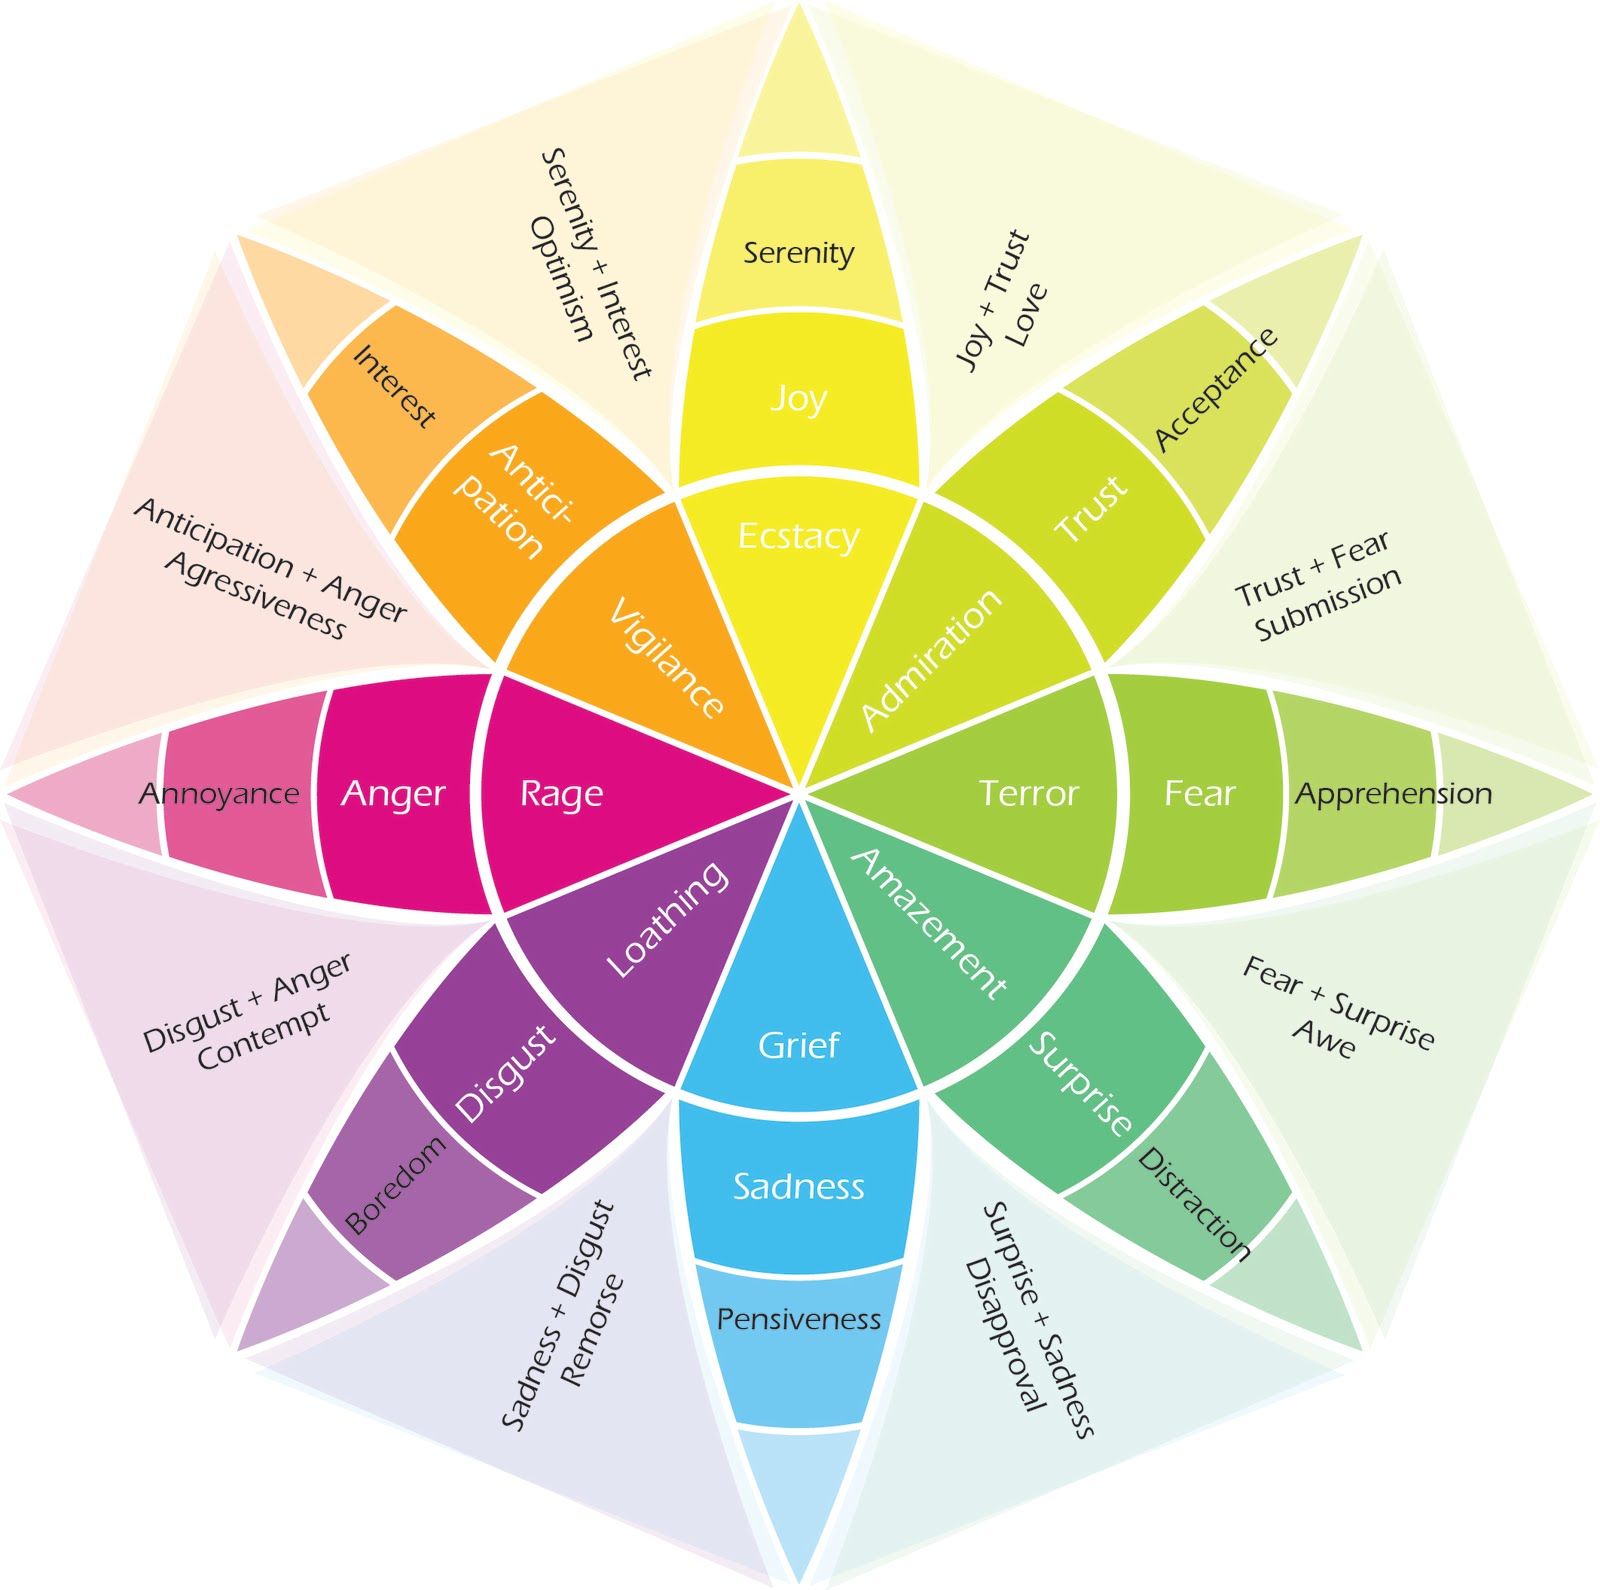
\includegraphics[width=\textwidth]{figures/plutchik_emotion_solid.jpg}}}$
        \label{fig_2d}
    \end{subfigure} \hspace{0.05\textwidth} %
    \begin{subfigure}[c]{0.25\textwidth}
        \centering

        $\vcenter{\hbox{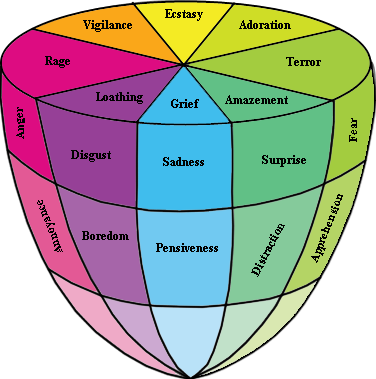
\includegraphics[width=\textwidth]{figures/plutchik_solid.png}}}$
        \label{fig_3d}
    \end{subfigure}
    \caption{A flattened and 3D view of the Emotion Structure}
    \label{fig_emotionsolid}
\end{figure}

\hrule

\paragraph{Source} \cite{robert1980emotion, block1957studies,
conte1976circumplex}

\paragraph{Depends On} --

\paragraph{Ref. By} \cref{C_ComplexEmotion}, \tref{T_GetEmotionStatePAD},
\tyref{TY_EmotionKind} \\\hrule\vspace{0.5mm}\hrule

~\newline

\noindent
\begin{minipage}{\textwidth}
    \renewcommand*{\arraystretch}{1.5}
    \begin{tabular}{| p{\colAwidth}  p{\colBwidth}|}
        \hline
        \rowcolor[gray]{0.9}
        \bf C\refstepcounter{conceptnum}\theconceptnum \label{C_ComplexEmotion}
        &\bf Mixing Emotions (PES) \\\hline
    \end{tabular}
\end{minipage}

\paragraph{Description} PES states that complex emotions are mixtures of
emotion types and intensity. It uses a colour wheel analogy to describe how to
mix them, where Emotion categories are hues and intensity is saturation.

In the PES structural model (\cref{C_EmotionStruct}), the tip of the cone has
no colour saturation whereas the circular plane is fully saturated with colour,
respectively representing no intensity and full intensity.
\\\hrule

\paragraph{Source} \cite{robert1980emotion}

\paragraph{Depends On} \cref{C_EmotionStruct}

\paragraph{Ref. By} \rref{R_MixingEmotionsPES}, \rref{R_PartitionEmotions}
\\\hrule\vspace{0.5mm}\hrule

\newpage\noindent
\begin{minipage}{\textwidth}
    \renewcommand*{\arraystretch}{1.5}
    \begin{tabular}{| p{\colAwidth}  p{\colBwidth}|}
        \hline
        \rowcolor[gray]{0.9}
        \bf C\refstepcounter{conceptnum}\theconceptnum
        \label{C_ComplexEmotions-CTE}
        &\bf ``Complex'' Emotions (CTE) \\\hline
    \end{tabular}
\end{minipage}

\paragraph{Description} CTE proposes that ``complex'' emotions are elaborations
of the emotion ``modes'' (\cref{C_Appraisal-CTE}), where the system ascribes
additional propositional meanings to it. For example, \textit{Disgust} is
typically called \textit{Contempt}, \textit{Disdain}, or \textit{Hatred} when
felt towards people instead of food, toxins, and/or
contamination~\citep[p.~60]{oatley1992best}. This also means that ``[e]motions
are in part socially constructed, but they are constructed around a biological
basis.''~\citep[p.~119]{oatley1992best}

This often requires a ``model of the self'' to draw meaning from, developed via
individual differences and culture. This model is also tied to the individual's
relationships with others (\cref{C_Relation-CTE}). \\\hrule

\paragraph{Source} \cite{oatley1987towards, oatley1992best}

\paragraph{Depends On} \cref{C_Appraisal-CTE}, \cref{C_Relation-CTE}

\paragraph{Ref. By} \tref{T_CalculateEmotionAcceptance},
\rref{R_MixingEmotionsCTE} \\\hrule\vspace{0.5mm}\hrule

~\newline

\noindent
\begin{minipage}{\textwidth}
    \renewcommand*{\arraystretch}{1.5}
    \begin{tabular}{| p{\colAwidth}  p{\colBwidth}|}
        \hline
        \rowcolor[gray]{0.9}
        \bf C\refstepcounter{conceptnum}\theconceptnum
        \label{C_PAD}
        &\bf PAD Space \\\hline
    \end{tabular}
\end{minipage}

\paragraph{Description} Based on studies in a variety of related fields with
the goal of quantifying different types of affective phenomena (e.g. emotion,
core affect, mood, personality), PAD describes describes a small set of nearly
orthogonal dimensions for analysing emotional states and behaviours, while as
relating them to other affect types and experiences. Points in this space can
represent different affective phenomena. The dimensions are present in all
affective reactions that are operative in any situation:
\begin{itemize}
    \item \textit{Pleasure} measures the positive-negative aspects of the
    emotion state (related to \textit{valence}),

    \item \textit{Arousal} is how alert and active the individual is in that
    state, and

    \item \textit{Dominance} is how much control the individual feels they have
    in that state.
\end{itemize}

The range of each dimension is $-1$ to $1$ representing mean ratings for
emotion terms. Means are based on ratings from $16$ to $31$ subjects,
transformed to the $-1$ to $1$ scale. Statistical significance---measured from
a mean of $0$ with $(p > 0.01)$---and standard deviations differ between
ratings.

Three dimensions are optimal for general characterizations and measurements of
emotional states, as two dimensions cannot distinguish between clusters of
affect and additional dimensions added little value to evaluations\\\hrule

\paragraph{Source} \cite{mehrabian1980basic, mehrabian1996pleasure}

\paragraph{Depends On} --

\paragraph{Ref. By} \tref{T_GetEmotionStatePAD}, \tyref{TY_PAD}
\\\hrule\vspace{0.5mm}\hrule

~\newpage

\noindent
\begin{minipage}{\textwidth}
    \renewcommand*{\arraystretch}{1.5}
    \begin{tabular}{| p{\colAwidth}  p{\colBwidth}|}
        \hline
        \rowcolor[gray]{0.9}
        \bf C\refstepcounter{conceptnum}\theconceptnum \label{C_Appraisal-CTE}
        &\bf Emotion Modes (CTE) \\\hline
    \end{tabular}
\end{minipage}

\paragraph{Description} CTE hypothesizes that a system can change its emotion
``mode'' (i.e. type) at plan junctures, identifiable by changes in the likely
success of a plan (\cref{C_Plans}). These junctures are assumed to be
distinctive and recurring. The system enters a ``mode'' based on the current
plan state and if/how goals (\cref{C_Goals}) are impacted, and form the basis
for other emotion ``types'' (see \cref{C_ComplexEmotions-CTE}).

\begin{table}[H]
    \centering
    \label{tab:cte_pattern}
    \renewcommand{\arraystretch}{1.2}
    \begin{tabular}{lll}
        \toprule
        \textbf{Emotion} & \textbf{Juncture of Current Plan} & \textbf{Next
        State} \\ \midrule

        \rowcolor[gray]{0.9}\textit{Happiness} & Sub-goals being achieved &
        Continue, modifying if needed \\

        \textit{Sadness} & Failure of a major plan or loss of an active goal &
        Do nothing/Search for a new plan \\

        \rowcolor[gray]{0.9}\textit{Anxiety} & Self-preservation goal
        threatened & Stop, Attend to Environment/Escape \\

        \textit{Anger} & Active plan frustrated & Try harder/Aggress \\

        \rowcolor[gray]{0.9}\textit{Disgust} & Gustatory goal violated & Reject
        substance/Withdraw \\

        \bottomrule
    \end{tabular}
\end{table}

CTE proposes that the emotion ``modes'' inhibit each other, and there might
also be conflicts that prevent the system from settling into a ``mode''. Being
in an emotion ``mode'' is a necessary---but not sufficient---condition to
experience emotion. A true emotion also requires the assignment of meaning to
the ``mode'' and the scheduling of voluntary actions. \\\hrule

\paragraph{Source} \cite{oatley1987towards, oatley1992best}

\paragraph{Depends On} \cref{C_Goals}, \cref{C_Plans}

\paragraph{Ref. By} \cref{C_ComplexEmotions-CTE}, \cref{C_EmOther},
\cref{C_EmIntensity-CTE}, \tref{T_CalculateEmotionGP}
\\\hrule\vspace{0.5mm}\hrule

~\newline

\noindent
\begin{minipage}{\textwidth}
    \renewcommand*{\arraystretch}{1.5}
    \begin{tabular}{| p{\colAwidth}  p{\colBwidth}|}
        \hline
        \rowcolor[gray]{0.9}
        \bf  C\refstepcounter{conceptnum}\theconceptnum \label{C_EmOther} & \bf
        ``Other Emotions''\\ \hline
    \end{tabular}
\end{minipage}

\paragraph{Description} Researchers continue to debate if \textit{Surprise} and
\textit{Interest} are ``emotions''. CTE is unsure of their status, but proposes
that:
\begin{itemize}
    \item \textit{Surprise} ``...is elicited by a sudden unexpected
    event...''~\citep[p.~33]{oatley1987towards}. This seems to align with the
    ``stopping'' behaviour tendencies that PES associates with
    \textit{Surprise}. Sudden, unexpected events cause \textit{Surprise}, and
    could represent an interruption and abrupt transition to another emotion
    ``mode'' (\cref{C_Appraisal-CTE})

    \item \textit{Interest} ``...implies sustained attention to certain external
    events''~\citep[p.~33]{oatley1987towards} (\cref{C_Attention}). This seems
    to align with the ``starting'' behaviour tendencies that PES associates
    with \textit{Interest}
\end{itemize}

Both descriptions imply that \textit{Surprise} and \textit{Interest} can
coexist with, or are part of, other emotion ``modes''.\\\hrule

\paragraph{Source} \cite{oatley1987towards, oatley1992best},
\cite{plutchik1984emotions}

\paragraph{Depends On} \cref{C_Appraisal-CTE}, \cref{C_Attention}

\paragraph{Ref. By} \tref{T_CalculateEmotionInterest},
\tref{T_CalculateEmotionSurprise}
\\\hrule\vspace{0.5mm}\hrule

~\newline

\noindent
\begin{minipage}{\textwidth}
    \renewcommand*{\arraystretch}{1.5}
    \begin{tabular}{| p{\colAwidth}  p{\colBwidth}|}
        \hline
        \rowcolor[gray]{0.9}
        \bf C\refstepcounter{conceptnum}\theconceptnum
        \label{C_EmIntensity-CTE}
        &\bf Emotion Intensity (CTE) \\\hline
    \end{tabular}
\end{minipage}

\paragraph{Description} Overall, emotion intensity is a relatively understudied
topic. CTE proposes that the intensity of an emotion (\cref{C_Emotion})
corresponds to how entrained the system is in a ``mode''
(\cref{C_Appraisal-CTE}) and to what degree it is ``locked into'' it. There
appear to be four determinant categories of emotion intensity evaluation:
\begin{itemize}
    \item How much the entity ``values'' affected internal conditions (e.g.
    goals),
    \item The ``seriousness'' or ``value'' of the event that affected those
    internal conditions,
    \item Contextual considerations of elements such as coping, support, and
    unexpectedness, and
    \item The entity's personality attributes that affect factors such as
    emotion response thresholds and dispositions towards different emotions.
\end{itemize}\hrule

\paragraph{Source} \cite{frijda1992complexity, oatley1987towards,
oatley1992best}

\paragraph{Depends On} \cref{C_Emotion}, \cref{C_Appraisal-CTE}

\paragraph{Ref. By} \tref{T_CalculateEmotionIntensity}
\\\hrule\vspace{0.5mm}\hrule

~\newline

\noindent
\begin{minipage}{\textwidth}
    \renewcommand*{\arraystretch}{1.5}
    \begin{tabular}{| p{\colAwidth}  p{\colBwidth}|}
        \hline
        \rowcolor[gray]{0.9}
        \bf  C\refstepcounter{conceptnum}\theconceptnum \label{C_EmDecay} & \bf
        Emotion Decay\\ \hline
    \end{tabular}
\end{minipage}

\paragraph{Description} Emotions (\cref{C_Emotion}) do not last
indefinitely---they dissipate after a time, implying the presence of an emotion
decay mechanism. This requires a specification of baseline values for each
emotion and as well as one or more decay functions. \\\hrule

\paragraph{Source} \cite{broekens2021emotion}

\paragraph{Depends On} \cref{C_Emotion}

\paragraph{Ref. By} \tref{T_DecayEmotionState} \\\hrule\vspace{0.5mm}\hrule

~\newline

\clearpage\noindent
\begin{minipage}{\textwidth}
    \renewcommand*{\arraystretch}{1.5}
    \begin{tabular}{| p{\colAwidth}  p{\colBwidth}|}
        \hline
        \rowcolor[gray]{0.9}
        \bf C\refstepcounter{conceptnum}\theconceptnum \label{C_Goals} & \bf
        Goals \\\hline
    \end{tabular}
\end{minipage}

\paragraph{Description} Goals compel systems to act in ways that achieve a
desired objective. They are essential for emotion processing, identifying what
elements of the current world state are relevant to an individual rather than
relying on properties of the environment alone. Entities use goals to know when
events impact them and by how much. Goals are also connected to emotions,
partially motivating emotion-driven behaviours.

PES describes goals as being in service to global adaptational problems,
whereas CTE view them as symbolic representations of possible environmental
states that a system wants to achieve. \\\hrule

\paragraph{Source} \cite{oxfordGoals}, \citet[p.~223]{broekens2016emotional},
\cite{robert1980emotion, oatley1987towards}, \citet[p.~208]{ortony2002making}

\paragraph{Depends On} --

\paragraph{Ref. By} \cref{C_Emotion}, \cref{C_Appraisal-CTE}, \cref{C_Plans},
\tref{T_CalculateEmotionGP}, \tyref{TY_Goal} \\\hrule\vspace{0.5mm}\hrule

~\newline

\noindent
\begin{minipage}{\textwidth}
    \renewcommand*{\arraystretch}{1.5}
    \begin{tabular}{| p{\colAwidth}  p{\colBwidth}|}
        \hline
        \rowcolor[gray]{0.9}
        \bf C\refstepcounter{conceptnum}\theconceptnum \label{C_Plans} & \bf
        Plans (CTE) \\\hline
    \end{tabular}
\end{minipage}

\paragraph{Description} CTE describes plans as sequences of transformations
between symbolic representations of possible environmental states, linking the
current state to a goal (\cref{C_Goals}). To ``make'' a plan is to create a
sequence of transformations, and to ``execute'' the plan is to enact the
sequence in the world.

A system forms plans with imperfect and incomplete knowledge of the
environment, and often only looks one or two steps ahead. \\\hrule

\paragraph{Source} \cite{oatley1987towards}

\paragraph{Depends On} \cref{C_Goals}

\paragraph{Ref. By} \cref{C_Appraisal-CTE}, \tref{T_CalculateEmotionGP},
\tyref{TY_Plan} \\\hrule\vspace{0.5mm}\hrule

~\newline

\noindent
\begin{minipage}{\textwidth}
    \renewcommand*{\arraystretch}{1.5}
    \begin{tabular}{| p{\colAwidth}  p{\colBwidth}|}
        \hline
        \rowcolor[gray]{0.9}
        \bf C\refstepcounter{conceptnum}\theconceptnum \label{C_Relation-CTE} &
        \bf Social Relationship \\\hline
    \end{tabular}
\end{minipage}

\paragraph{Description} CTE states that many emotions are social, occurring in
the course of one's relationships with others. This allows them to construct
mutual plans to coordinate the actions of multiple actors, which also requires
each actor to have a ``model of the self''.

The emotion of \textit{Acceptance} (i.e. \textit{Trust})---an elementary
component of social life---in PES also implies the existence of relationships
with others. ``Affective trust'' builds on past experiences with, feelings of
security, confidence, and satisfaction towards, and the perceived level of
selfless concern demonstrated by a partner regardless of what the future holds.
The biological basis of affective trust might lie in social attachment and
affiliation due to the role of oxytocin.

A social relationship is a representation of the history shared between the
individual and another person, entity, or thing. They can be established
implicitly based on precedents and customs (i.e. culture). \\\hrule

\paragraph{Source} \cite{oatley1987towards, oxfordTrust, rempel1985trust}

\paragraph{Depends On} --

\paragraph{Ref. By} \cref{C_ComplexEmotions-CTE},
\tref{T_CalculateEmotionAcceptance}, \tyref{TY_Relation-CTE}
\\\hrule\vspace{0.5mm}\hrule

~\newline

\noindent
\begin{minipage}{\textwidth}
    \renewcommand*{\arraystretch}{1.5}
    \begin{tabular}{| p{\colAwidth}  p{\colBwidth}|}
        \hline
        \rowcolor[gray]{0.9}
        \bf C\refstepcounter{conceptnum}\theconceptnum \label{C_Attention} &
        \bf Attention \\\hline
    \end{tabular}
\end{minipage}

\paragraph{Description} Attention is a set of mechanisms that allow a
limited-capacity system to select salient or goal-relevant information. These
mechanisms might work in parallel. Behavioural effects of attention vary
between systems, partially due to personality. \\\hrule

\paragraph{Source} \cite{oxfordAttention}

\paragraph{Depends On} --

\paragraph{Ref. By} \cref{C_EmOther}, \tyref{TY_Attention}
\\\hrule\vspace{0.5mm}\hrule

\newpage

\subsubsection{Theoretical Models}\label{sec_theoretical}

These models refine the Conceptual Models (Section~\ref{sec_conceptual}) using
natural language to improve their precision. This is a necessary step for
reducing ambiguity by explicitly stating how the primary sources are understood
and showing how they relate to the mathematically-defined Data Types
(Section~\ref{sec_typedefs}) and Instance Models (Section~\ref{sec_instance})
using Assumptions (Section~\ref{sec_assumptions}).

~\newline\noindent
\begin{minipage}{\textwidth}
    \renewcommand*{\arraystretch}{1.5}
    \begin{tabular}{| p{\colAwidth}  p{\colBwidth}|}
        \hline
        \rowcolor[gray]{0.9}
        \bf T\refstepcounter{theorynum}\thetheorynum
        \label{T_CalculateEmotionGP} &
        \bf Evaluate Emotion Kind from Goals and Plans \\
        \hline
    \end{tabular}
\end{minipage}

\paragraph{Description} The emotion kinds (``modes'') that CTE defines
(\cref{C_Appraisal-CTE})---\textit{Happiness}, \textit{Sadness}, \textit{Fear},
\textit{Anger}, \textit{Disgust}---in terms of goals (\cref{C_Goals}) and plans
(\cref{C_Plans}) can be re-conceptualized as follows:
\begin{itemize}
    \item \textit{Joy} (\textit{Happiness}) occurs when an action moves an
    entity closer to achieving a goal, assuming that each such action is a goal
    itself (i.e. a ``sub-goal'' of the goal, \aref{A_Subgoal})

    \item \textit{Sadness} occurs when an entity has a plan where a next step
    is impossible to achieve (i.e. ``failure of a plan''), or a goal becomes
    impossible to achieve (i.e. ``loss of a goal'')

    \item \textit{Fear} (\textit{Anxiety}) occurs when there is a threat to
    self-preservation (i.e. ``self-preservation goal threatened''), which
    requires a prediction about a future world state based on the current world
    state and an action that could change it

    \item \textit{Anger} occurs when an entity has a plan where the next step
    cannot be reached after an intentional action to achieve it, but there are
    one or more other actions that can (i.e. the plan is ``frustrated'' because
    it is still feasible, but it had to change to remain so)

    \item \textit{Disgust} occurs when an entity has been ``contaminated'' or
    encounters ``contaminated'' substances that it wants to avoid (i.e.
    ``gustatory goal violated'')
\end{itemize}

It is assumed that a single goal can trigger more than one emotion
(\aref{A_Goal2Emotion}) and they all contribute to a single emotion state
(\aref{A_OneState}).

Emotion intensity is evaluated separately (\aref{A_EmotionTypeIntensity}, see
\tref{T_CalculateEmotionIntensity}). The emotions \textit{Surprise},
\textit{Interest}, and \textit{Acceptance} are evaluated differently because
they are not part of CTE's primary emotions (\aref{A_AppraisalProcess}, see
\tref{T_CalculateEmotionSurprise}, \tref{T_CalculateEmotionInterest}, and
\tref{T_CalculateEmotionAcceptance} respectively). \\\hrule

\paragraph{Sources} --

\paragraph{Depends On} \aref{A_Subgoal}, \aref{A_Goal2Emotion},
\aref{A_OneState}, \aref{A_EmotionTypeIntensity},
\aref{A_AppraisalProcess}, \cref{C_Appraisal-CTE}, \cref{C_Goals},
\cref{C_Plans}

\paragraph{Ref. By} \iref{IM_CalculateEmotionGP} \\\hrule\vspace{0.5mm}\hrule

~\newpage\noindent
\begin{minipage}{\textwidth}
    \renewcommand*{\arraystretch}{1.5}
    \begin{tabular}{| p{\colAwidth}  p{\colBwidth}|}
        \hline
        \rowcolor[gray]{0.9}
        \bf T\refstepcounter{theorynum}\thetheorynum
        \label{T_CalculateEmotionIntensity} &
        \bf Evaluate Emotion Intensity \\
        \hline
    \end{tabular}
\end{minipage}

\paragraph{Description} Emotion intensity (\cref{C_EmIntensity-CTE}) is
proportional to the force causing an emotion state (``entrained'') and how
fixed or non-adjustable that force is (``locked in''). This could be related to
the degree that something impacts a goal (\aref{A_Goal2Intensity})---either a
stand-alone goal or as part of a plan (i.e. a ``sub-goal'')---such that an
entity would want to maintain the momentum caused by an emotion ``mode'' as
long as that goal is affected. \\\hrule

\paragraph{Sources} --

\paragraph{Depends On} \aref{A_Goal2Intensity}, \cref{C_EmIntensity-CTE}

\paragraph{Ref. By} \tyref{TY_EmotionIntensity},
\iref{IM_CalculateEmotionIntensity} \\\hrule\vspace{0.5mm}\hrule

~\newline

\noindent
\begin{minipage}{\textwidth}
    \renewcommand*{\arraystretch}{1.5}
    \begin{tabular}{| p{\colAwidth}  p{\colBwidth}|}
        \hline
        \rowcolor[gray]{0.9}
        \bf T\refstepcounter{theorynum}\thetheorynum
        \label{T_CalculateEmotionSurprise} &
        \bf Evaluate \textit{Surprise} Emotion and Intensity \\
        \hline
    \end{tabular}
\end{minipage}

\paragraph{Description} An ``interruption and abrupt transition'' to a
different emotion state elicits \textit{Surprise} (\cref{C_EmOther}). This
suggests that it occurs when there is a large, rapid change in emotion
intensity (\aref{A_Surprise}), and/or there the emotion state recently changed
and it is changing again (``sudden, unexpected event'', \aref{A_Surprise2}).

For intensity, this implies that it is inversely proportional to time such that
less time it takes for the emotion intensity change to occur and/or between the
recently changed emotion state and the current change to a ``new'' emotion
state creates a higher intensity response. Intensity rapidly decreases as time
elapses. \\\hrule

\paragraph{Sources} --

\paragraph{Depends On} \aref{A_Surprise}, \aref{A_Surprise2}, \cref{C_EmOther}

\paragraph{Ref. By} \tyref{TY_EmotionIntensity},
\iref{IM_CalculateEmotionSurpriseElicit}, \iref{IM_CalculateEmotionSurprise}
\\\hrule\vspace{0.5mm}\hrule

~\newline

\noindent
\begin{minipage}{\textwidth}
    \renewcommand*{\arraystretch}{1.5}
    \begin{tabular}{| p{\colAwidth}  p{\colBwidth}|}
        \hline
        \rowcolor[gray]{0.9}
        \bf T\refstepcounter{theorynum}\thetheorynum
        \label{T_CalculateEmotionInterest} &
        \bf Evaluate \textit{Interest} Emotion and Intensity \\
        \hline
    \end{tabular}
\end{minipage}

\paragraph{Description} ``Sustained attention to certain external events''
elicits \textit{Interest} (\cref{C_EmOther}), implying that it occurs when an
entity is focused on the same thing (e.g. task, another entity) for an extended
period of time (\aref{A_Interest}). This suggests that there is a ``baseline''
amount of attention/time paid to something before it triggers
\textit{Interest}, which can differ between foci.

For intensity, this implies that it is proportional to the amount of time spent
focused on the same thing and relative to the ``baseline'' time spent. \\\hrule

\paragraph{Sources} --

\paragraph{Depends On} \aref{A_Interest}, \cref{C_EmOther}

\paragraph{Ref. By} \tyref{TY_EmotionIntensity},
\iref{IM_CalculateEmotionInterestElicit}, \iref{IM_CalculateEmotionInterest}
\\\hrule\vspace{0.5mm}\hrule

~\newline

\noindent
\begin{minipage}{\textwidth}
    \renewcommand*{\arraystretch}{1.5}
    \begin{tabular}{| p{\colAwidth}  p{\colBwidth}|}
        \hline
        \rowcolor[gray]{0.9}
        \bf T\refstepcounter{theorynum}\thetheorynum
        \label{T_CalculateEmotionAcceptance} &
        \bf Evaluate \textit{Acceptance} Emotion and Intensity \\
        \hline
    \end{tabular}
\end{minipage}

\paragraph{Description} Taking \textit{Acceptance} as a ``complex'' emotion
(\cref{C_ComplexEmotions-CTE}), it can be defined as \textit{Joy}
(\textit{Happiness}) elaborated with information about social relationships
(\cref{C_Relation-CTE}) such that an entity experiences \textit{Acceptance}
when it attributes a state of \textit{Joy} to another entity that they have an
established relationship with (\aref{A_Acceptance}). An entity might also
establish a relationship with another entity that is attributed with causing
the state, which would also elicit \textit{Acceptance}.

For intensity, this implies that it is proportional to the intensity of
\textit{Joy} and the strength of the relationship with the entity that the
state is attributed to. \\\hrule

\paragraph{Sources} \citet[p.~178--179]{oatley1992best}

\paragraph{Depends On} \aref{A_Acceptance}, \cref{C_ComplexEmotions-CTE},
\cref{C_Relation-CTE}

\paragraph{Ref. By} \tyref{TY_EmotionIntensity},
\iref{IM_CalculateEmotionAcceptanceElicit},
\iref{IM_CalculateEmotionAcceptance} \\\hrule\vspace{0.5mm}\hrule

~\newline

\noindent
\begin{minipage}{\textwidth}
    \renewcommand*{\arraystretch}{1.5}
    \begin{tabular}{| p{\colAwidth}  p{\colBwidth}|}
        \hline
        \rowcolor[gray]{0.9}
        \bf T\refstepcounter{theorynum}\thetheorynum
        \label{T_DecayEmotionState} &
        \bf Decaying Emotion State \\
        \hline
    \end{tabular}
\end{minipage}

\paragraph{Description} Emotion decay (\cref{C_EmDecay}) is a function of time
such that the emotion state returns to its ``equilibrium'' intensities as time
progresses. It is assumed that:
\begin{itemize}
    \item The speed that intensities return to ``equilibrium'' are assumed to
    be functions of distance such that larger differences between an intensity
    and its ``equilibrium'' cause larger changes in intensity
    (\aref{A_DecaySpeed})

    \item Each emotion kind has its own ``equilibrium'' value
    (\aref{A_Equilibrium}) and can decay at different rates (\aref{A_DecayRate})

    \item Decay rates and equilibrium values can differ between entities
    (\aref{A_DecayUnique})
\end{itemize}
\hrule

\paragraph{Sources} --

\paragraph{Depends On} \aref{A_DecaySpeed}, \aref{A_Equilibrium},
\aref{A_DecayRate}, \aref{A_DecayUnique}, \cref{C_EmDecay}

\paragraph{Ref. By} \tyref{TY_EmotionDecay}, \tyref{TY_EmotionDecayState},
\iref{IM_DecayEmotionState} \\\hrule\vspace{0.5mm}\hrule

~\clearpage

\noindent
\begin{minipage}{\textwidth}
    \renewcommand*{\arraystretch}{1.5}
    \begin{tabular}{| p{\colAwidth}  p{\colBwidth}|}
        \hline
        \rowcolor[gray]{0.9}
        \bf T\refstepcounter{theorynum}\thetheorynum
        \label{T_GetEmotionStatePAD} &
        \bf Getting an Emotion State as a PAD Point \\
        \hline
    \end{tabular}
\end{minipage}

\paragraph{Description} Assuming that an entity can only occupy one point in
PAD Space at any given time (\aref{A_OnePADPoint}), the intensities for each
discrete emotion in an emotion state must be combined into a single value for
each dimension in the space. This requires reference points for each emotion
type in PES because it defines the emotion state structure
(\cref{C_EmotionStruct}) that emotion intensities are mapped to.

In both theories, laypeople evaluated emotion terms for their contents. In both
experiments, the laypeople were likely from the same age group (university
undergraduates, college and graduate students), likely from the United States
(in the case of PAD, Californian), and likely to have participated in the
experiments around the same time given the publishing year of the work (1980).
Therefore, it is reasonable to assume that the meaning of the terms in PES and
PAD Space would be judged to be identical or nearly identical to each other by
the same laypeople (\aref{A_EmotionTerms}).

The circumplex representing the relative similarity of emotion term
meanings~\citep[p.~170]{robert1980emotion} was divided into ranges,
representing what language laypeople typical describe PES emotion kinds with.
Gaps between areas are small (0.3\textdegree{} at least, 7.3\textdegree{} at
most), so they are ignored. The list of 145 emotion terms from PES and 151 from
PAD~\citep[p.~42--45]{mehrabian1980basic} were compared for common terms, which
were listed by PES emotion kind. An emotion term was selected from each list
based on its similarity to the emotion kind label. There was no such term for
\textit{Acceptance}, so \progname{} uses the term closest to the mean range on
the circumplex (i.e. ``Affectionate''). Where possible, emotion terms that had
statistical significance ($p < 0.01$) for all dimensions define reference
points (e.g. \textit{Astonished} is statistically significant on all three
dimensions, whereas \textit{Surprised} is only significant for two). All terms
achieved significance for \textit{pleasure} and \textit{arousal}.
\textit{Interested} and \textit{Disgust} are not statistically significant for
\textit{dominance}.

An emotion term's \textit{pleasure}, \textit{arousal}, and \textit{dominance}
mean values (\cref{C_PAD}) form a reference point. Number of ratings and
standard deviation do not affect reference points (\aref{A_PADStats}).

\begin{table}[H]
    \centering
    \renewcommand{\arraystretch}{1.2}
    \begin{tabular}{ccccc}
        \toprule
        \multicolumn{2}{c}{\textbf{PES}} &  &  & \\
        $k \in \emotionkindstype$ & Range on Circumplex (\textdegree) & Term  &
        Circumplex Location (\textdegree) & PAD Ref.~\# \\
        \midrule

        \rowcolor[gray]{0.9}\textit{Fear} & $[65.0, 86.0]$ & Terrified & 75.5 &
        102 \\

        \textit{Anger} & $[200.6, 249.0]$ & Angry & 212.0 & 82 \\

        \rowcolor[gray]{0.9}\textit{Sadness} & $[88.3, 138.0]$ & Sad & 108.5 &
        151 \\

        \textit{Joy} & $[323.4, 338.3]$ & Joyful & 323.4 & 20 \\

        \rowcolor[gray]{0.9}\textit{Interest} & $[249.7, 322.4]$ & Interested &
        315.7 & 8 \\

        \textit{Surprise} & $[138.3, 156.7]$ & Astonished & 148.0 & 74 \\

        \rowcolor[gray]{0.9}\textit{Disgust} & $[160.3, 193.7]$ & Disgusted &
        161.3 & 75 \\

        \textit{Acceptance} & $[340.7, 57.7]$ & Affectionate & 52.3 & 34 \\

        \bottomrule
    \end{tabular}
\end{table}

\hrule

\paragraph{Sources} \citet[p.~40, 42--45]{mehrabian1980basic},
\citet[p.~159, 170]{robert1980emotion}, \cite{conte1976circumplex}

\paragraph{Depends On} \aref{A_OnePADPoint}, \aref{A_EmotionTerms},
\aref{A_PADStats}, \cref{C_EmotionStruct}, \cref{C_PAD}

\paragraph{Ref. By} \iref{IM_GetEmotionStatePAD} \\\hrule\vspace{0.5mm}\hrule

\newpage

\subsubsection{General Definitions}\label{sec_gendef}

No additional information is required to build the data definitions.

\subsubsection{Data Definitions}\label{sec_datadef}

No data definitions are needed.

\newpage

\subsubsection{Data Types}\label{sec_typedefs}
This section defines types for realizing \progname{}'s Instance Models
(Section~\ref{sec_instance}). Data types also allow for type checking to verify
and enforce constraints (Section~\ref{sec_DataConstraints}), and defining model
interfaces.

Data types \tyref{TY_Time}, \tyref{TY_WorldState}, \tyref{TY_WorldStateChange},
\tyref{TY_DistanceBetweenWorldStates},
\tyref{TY_DistanceBetweenWorldStatesChange}, \tyref{TY_Goal}, \tyref{TY_Plan},
\tyref{TY_Attention}, and \tyref{TY_Relation-CTE} are APIs for users to
implement for their specific needs.
\begin{itemize}
    \item \tyref{TY_Time}, \tyref{TY_WorldState}, \tyref{TY_WorldStateChange},
    \tyref{TY_DistanceBetweenWorldStates},
    \tyref{TY_DistanceBetweenWorldStatesChange}, and \tyref{TY_Goal} are
    mandatory

    \item \tyref{TY_Plan} is optional, but necessary for \textit{Anger}

    \item \tyref{TY_Attention} is optional, but necessary for \textit{Interest}

    \item \tyref{TY_Relation-CTE} is optional, but necessary for
    \textit{Acceptance}
\end{itemize}

~\newline\noindent
\begin{minipage}{\textwidth}
    \renewcommand*{\arraystretch}{1.5}
    \begin{tabular}{| p{\colAwidth}  p{\colBwidth}|}
        \hline
        \rowcolor[gray]{0.9}
        \bf TY\refstepcounter{typenum}\thetypenum
        \label{TY_Time} & \bf Type of Time and Delta Time \\
        \hline
    \end{tabular}

    \renewcommand*{\arraystretch}{1.5}
    \begin{tabular}{ p{\colAwidth}  p{\colBwidth}}
        \bf Symbol & $\timetype, \deltatimetype$ \\

        \bf Type & -- \\\hline
    \end{tabular}
\end{minipage}

\paragraph{Description} Time is an abstract type that is linearly ordered. A
Delta Time is the difference between two Time values. \\\hrule

\paragraph{Sources} --

\paragraph{Depends On} --

\paragraph{Ref. By} \tyref{TY_Emotion}, \tyref{TY_Attention},
\iref{IM_CalculateEmotionSurpriseElicit}, \iref{IM_CalculateEmotionSurprise},
\iref{IM_DecayEmotionState}, \iref{IM_UpdateEmotion},
\iref{IM_GetEmotionState}, \iref{IM_DecayEmotion}, \rref{R_TimeType}
\\\hrule\vspace{0.5mm}\hrule

~\newline

\noindent
\begin{minipage}{\textwidth}
    \renewcommand*{\arraystretch}{1.5}
    \begin{tabular}{| p{\colAwidth}  p{\colBwidth}|}
        \hline
        \rowcolor[gray]{0.9}
        \bf TY\refstepcounter{typenum}\thetypenum
        \label{TY_EmotionIntensity} & \bf Type of Emotion Intensity \\
        \hline
    \end{tabular}

    \renewcommand*{\arraystretch}{1.5}
    \begin{tabular}{ p{\colAwidth}  p{\colBwidth}}
        \bf Symbol & $\emotionintensitytype$ \\

        \bf Type & $ \mathbb{R}_{\geq0} $
        \\\hline
    \end{tabular}
\end{minipage}

\paragraph{Description} Emotion intensity (\tref{T_CalculateEmotionIntensity},
\tref{T_CalculateEmotionSurprise}, \tref{T_CalculateEmotionInterest},
\tref{T_CalculateEmotionAcceptance}) is a real, non-negative value
(\aref{A_PositiveIntensity}). \\\hrule

\paragraph{Sources} --

\paragraph{Depends On} \aref{A_PositiveIntensity},
\tref{T_CalculateEmotionIntensity}, \tref{T_CalculateEmotionSurprise},
\tref{T_CalculateEmotionInterest}, \tref{T_CalculateEmotionAcceptance}

\paragraph{Ref. By} \tyref{TY_DeltaIntensity}, \tyref{TY_EmotionState},
\tyref{TY_EmotionDecayState}, \iref{IM_CalculateEmotionAcceptanceElicit},
\iref{IM_DecayEmotionState}, \iref{IM_UpdateEmotionState},
\iref{IM_UpdateEmotionState2}, \rref{R_IntensityTypeUse},
\rref{R_MixingEmotionsPES}, \rref{R_PartitionEmotions}
\\\hrule\vspace{0.5mm}\hrule

~\newline

\noindent
\begin{minipage}{\textwidth}
    \renewcommand*{\arraystretch}{1.5}
    \begin{tabular}{| p{\colAwidth}  p{\colBwidth}|}
        \hline
        \rowcolor[gray]{0.9}
        \bf TY\refstepcounter{typenum}\thetypenum
        \label{TY_DeltaIntensity} & \bf Type of Emotion Intensity Change \\
        \hline
    \end{tabular}

    \renewcommand*{\arraystretch}{1.5}
    \begin{tabular}{ p{\colAwidth}  p{\colBwidth}}
        \bf Symbol & $ \responsestrength $ \\

        \bf Type & $ \mathbb{R} $ \\\hline
    \end{tabular}
\end{minipage}

\paragraph{Description} A change in emotion intensity represents the magnitude
of a difference to be applied to an emotion intensity
(\tyref{TY_EmotionIntensity}). It is a real value because:
\begin{itemize}
    \item Emotion intensity can both increase and decrease, and

    \item The magnitude of a change should not be pre-emptively constrained to
    fit the type of $\emotionintensitytype$ in case $\responsestrength$ has
    other uses
\end{itemize} \hrule

\paragraph{Sources} --

\paragraph{Depends On} \tyref{TY_EmotionIntensity}

\paragraph{Ref. By} \iref{IM_CalculateEmotionIntensity},
\iref{IM_CalculateEmotionSurprise}, \iref{IM_CalculateEmotionInterest},
\iref{IM_CalculateEmotionAcceptance}, \iref{IM_UpdateEmotionState},
\rref{R_IntensityChangeType} \\\hrule\vspace{0.5mm}\hrule

~\newline

\noindent
\begin{minipage}{\textwidth}
    \renewcommand*{\arraystretch}{1.5}
    \begin{tabular}{| p{\colAwidth}  p{\colBwidth}|}
        \hline
        \rowcolor[gray]{0.9}
        \bf TY\refstepcounter{typenum}\thetypenum
        \label{TY_EmotionDecay} & \bf Type of Emotion Intensity Decay Rate \\
        \hline
    \end{tabular}

    \renewcommand*{\arraystretch}{1.5}
    \begin{tabular}{ p{\colAwidth}  p{\colBwidth}}
        \bf Symbol & $ \emotiondecaytype $ \\

        \bf Type & $ \mathbb{R}_{>0} $ \\\hline
    \end{tabular}
\end{minipage}

\paragraph{Description} Emotion decay rate (\tref{T_DecayEmotionState}) is a
real-valued, strictly positive constant. It is equivalent to the spring
constant $k_s$ in a damped harmonic oscillator, which is always strictly
positive. \\\hrule

\paragraph{Sources}
{\small\url{https://en.wikipedia.org/wiki/Harmonic_oscillator#Damped_harmonic_oscillator}}

\paragraph{Depends On} \tref{T_DecayEmotionState}

\paragraph{Ref. By} \tyref{TY_EmotionDecayState}, \iref{IM_DecayEmotionState},
\rref{R_IntensityDecayType} \\\hrule\vspace{0.5mm}\hrule

~\newline

\noindent
\begin{minipage}{\textwidth}
    \renewcommand*{\arraystretch}{1.5}
    \begin{tabular}{| p{\colAwidth}  p{\colBwidth}|}
        \hline
        \rowcolor[gray]{0.9}
        \bf TY\refstepcounter{typenum}\thetypenum
        \label{TY_EmotionKind} & \bf Type of Emotion Kinds \\
        \hline
    \end{tabular}

    \renewcommand*{\arraystretch}{1.5}
    \begin{tabular}{ p{\colAwidth}  p{\colBwidth}}
        \bf Symbol & $\emotionkindstype$ \\

        \bf Type & $ \left< \mFear, \mAnger, \mSadness, \mJoy, \mInterest,
        \mSurprise, \mDisgust, \mTrust \right> $ \\

        \bf Invariants & $\bullet$ $\emotionkindstype$ is finite and ordered

        $\bullet$ Each element of $\emotionkindstype$ is uniquely paired with
        exactly one other element that is not itself \\
        \hline
    \end{tabular}
\end{minipage}

\paragraph{Description} Emotion kinds is an enumeration representing the
primary emotion kinds from PES (\cref{C_EmotionStruct}). ``Opposing'' emotions
as defined in PES are enforced via the invariant regarding unique pairings.
\\\hrule

\paragraph{Sources} --

\paragraph{Depends On} \cref{C_EmotionStruct}

\paragraph{Ref. By} \tyref{TY_EmotionState}, \tyref{TY_EmotionDecayState},
\iref{IM_CalculateEmotionGP}, \iref{IM_UpdateEmotionState},
\iref{IM_UpdateEmotionState2}, \iref{IM_DecayEmotion},
\iref{IM_GetEmotionStatePAD}, \rref{R_EmotionKindsType},
\rref{R_MixingEmotionsPES}, \rref{R_PartitionEmotions},
\rref{R_MixingEmotionsCTE} \\\hrule\vspace{0.5mm}\hrule

~\newline

\noindent
\begin{minipage}{\textwidth}
    \renewcommand*{\arraystretch}{1.5}
    \begin{tabular}{| p{\colAwidth}  p{\colBwidth}|}
        \hline
        \rowcolor[gray]{0.9}
        \bf TY\refstepcounter{typenum}\thetypenum
        \label{TY_EmotionState} & \bf Type of Emotion State \\
        \hline
    \end{tabular}

    \renewcommand*{\arraystretch}{1.5}
    \begin{tabular}{ p{\colAwidth}  p{\colBwidth}}
        \bf Symbol & $\emotionstatetype$ \\

        \bf Type & $ \left\{ \mathtt{intensities} : \emotionkindstype
        \rightarrow \emotionintensitytype, \mathtt{max} : \emotionkindstype
        \rightarrow \emotionintensitytype \right\}  $ \\

        \bf Invariant & $\forall k \in \emotionkindstype \Rightarrow 0 \leq
        \mathtt{intensities}(k) \leq \mathtt{max}(k) $
        (\aref{A_LimitIntensity}) \\
        \hline
    \end{tabular}
\end{minipage}

\paragraph{Description} An emotion state is a record with:
\begin{itemize}

    \item An intensity function $\mathtt{intensities}$ mapping each element in
    $\emotionkindstype$ (\tyref{TY_EmotionKind}) to an intensity value
    $\emotionintensitytype$ (\tyref{TY_EmotionIntensity})

    \item An intensity function $\mathtt{max}$ mapping each element in
    $\emotionkindstype$ (\tyref{TY_EmotionKind}) to a maximum intensity value
    $\emotionintensitytype$ (\tyref{TY_EmotionIntensity})

\end{itemize}

The invariant ensures that emotion intensity is finite
(\aref{A_LimitIntensity}). Each element in $\emotionstatetype$ is independent
(\aref{A_EmotionPairs}, \cref{C_Emotion}).\\\hrule

\paragraph{Sources} --

\paragraph{Depends On} \aref{A_LimitIntensity}, \aref{A_EmotionPairs},
\cref{C_Emotion}, \tyref{TY_EmotionIntensity}, \tyref{TY_EmotionKind}

\paragraph{Ref. By} \tyref{TY_Emotion}, \iref{IM_UpdateEmotionState2},
\iref{IM_UpdateEmotion}, \iref{IM_GetEmotionState}, \iref{IM_DecayEmotion},
\iref{IM_GetEmotionStatePAD}, \rref{R_EmotionStateType}
\\\hrule\vspace{0.5mm}\hrule

~\newline

\noindent
\begin{minipage}{\textwidth}
    \renewcommand*{\arraystretch}{1.5}
    \begin{tabular}{| p{\colAwidth}  p{\colBwidth}|}
        \hline
        \rowcolor[gray]{0.9}
        \bf TY\refstepcounter{typenum}\thetypenum
        \label{TY_EmotionDecayState} & \bf Type of Emotion State Decay \\
        \hline
    \end{tabular}

    \renewcommand*{\arraystretch}{1.5}
    \begin{tabular}{ p{\colAwidth}  p{\colBwidth}}
        \bf Symbol & $ \emotionstatedecaytype $ \\

        \bf Type & $ \left\{ \mathtt{equilibrium} : \emotionkindstype
        \rightarrow \emotionintensitytype, \mathtt{decayRates} :
        \emotionkindstype \rightarrow \emotiondecaytype \right\} $ \\

        \bf Invariants & Given an $es : \emotionstatedecaytype$,
        $\left(\mathlarger\sum_{k \in\emotionkindstype}
        es.\mathtt{equilibrium}\left(k\right)\right) > 0$
        (\aref{A_PositiveIntensity})
        \vspace*{2mm}\\\hline
    \end{tabular}
\end{minipage}

\paragraph{Description} Emotion state decay (\tref{T_DecayEmotionState}) is a
record that has:
\begin{itemize}
    \item An equilibrium intensity function $\mathtt{equilibrium}$ mapping each
    element in $\emotionkindstype$ (\tyref{TY_EmotionKind}) to a ``stable''
    intensity value $\emotionintensitytype$ (\tyref{TY_EmotionIntensity}), and

    \item An emotion decay rate function $\mathtt{decayRates}$ mapping each
    element in $\emotionkindstype$ to a rate of decay $\emotiondecaytype$
    (\tyref{TY_EmotionDecay}) to use when returning to them equilibrium values.
\end{itemize}

The equilibrium function is not constantly zero (\aref{A_PositiveIntensity}).
\\\hrule

\paragraph{Sources} --

\paragraph{Depends On} \aref{A_PositiveIntensity}, \tref{T_DecayEmotionState},
\tyref{TY_EmotionIntensity}, \tyref{TY_EmotionDecay}, \tyref{TY_EmotionKind}

\paragraph{Ref. By} \iref{IM_DecayEmotion}, \rref{R_EmotionDecayStateType}
\\\hrule\vspace{0.5mm}\hrule

~\newline

\noindent
\begin{minipage}{\textwidth}
    \renewcommand*{\arraystretch}{1.5}
    \begin{tabular}{| p{\colAwidth}  p{\colBwidth}|}
        \hline
        \rowcolor[gray]{0.9}
        \bf TY\refstepcounter{typenum}\thetypenum
        \label{TY_Emotion} & \bf Type of Emotion \\
        \hline
    \end{tabular}

    \renewcommand*{\arraystretch}{1.5}
    \begin{tabular}{ p{\colAwidth}  p{\colBwidth}}
        \bf Symbol & $\emotiontype$\\

        \bf Type & $ \timetype \rightarrow \emotionstatetype $ \\

        \hline
    \end{tabular}
\end{minipage}

\paragraph{Description} Emotion $\emotiontype$ (\cref{C_Emotion}) is the
assignment of an emotion state $\emotionstatetype$ (\tyref{TY_EmotionState}) to
each instant in time $t : \timetype$ (\tyref{TY_Time}).
\\\hrule

\paragraph{Sources} --

\paragraph{Depends On} \cref{C_Emotion}, \tyref{TY_Time},
\tyref{TY_EmotionState}

\paragraph{Ref. By} \iref{IM_UpdateEmotion}, \iref{IM_GetEmotionState},
\iref{IM_DecayEmotion}, \rref{R_EmotionType} \\\hrule\vspace{0.5mm}\hrule

~\newline

\noindent
\begin{minipage}{\textwidth}
    \renewcommand*{\arraystretch}{1.5}
    \begin{tabular}{| p{\colAwidth}  p{\colBwidth}|}
        \hline
        \rowcolor[gray]{0.9}
        \bf TY\refstepcounter{typenum}\thetypenum
        \label{TY_PAD} & \bf Type of PAD Point \\
        \hline
    \end{tabular}

    \renewcommand*{\arraystretch}{1.5}
    \begin{tabular}{ p{\colAwidth}  p{\colBwidth}}
        \bf Symbol & $\padpoint$ \\

        \bf Type & $ \left( \mathtt{pleasure} : \left[-1,1\right] \subset
        \mathbb{R}, \mathtt{arousal} : \left[-1,1\right] \subset \mathbb{R},
        \mathtt{dominance} : \left[-1,1\right] \subset \mathbb{R} \right) $ \\

        \hline
    \end{tabular}
\end{minipage}

\paragraph{Description} A PAD point (\cref{C_PAD}) is a 3-tuple representing a
point in the space defined by the \textit{pleasure} ($P$), \textit{arousal}
($A$), and \textit{dominance} ($D$) dimensions (\tref{T_GetEmotionStatePAD}).
\\\hrule

\paragraph{Sources} \cite{mehrabian1980basic}

\paragraph{Depends On} \cref{C_PAD}

\paragraph{Ref. By} \iref{IM_GetEmotionStatePAD}, \rref{R_PADPointType}
\\\hrule\vspace{0.5mm}\hrule

~\newline

\noindent
\begin{minipage}{\textwidth}
    \renewcommand*{\arraystretch}{1.5}
    \begin{tabular}{| p{\colAwidth}  p{\colBwidth}|}
        \hline
        \rowcolor[gray]{0.9}
        \bf TY\refstepcounter{typenum}\thetypenum
        \label{TY_WorldState} & \bf Type of Game World State \\
        \hline
    \end{tabular}

    \renewcommand*{\arraystretch}{1.5}
    \begin{tabular}{ p{\colAwidth}  p{\colBwidth}}
        \bf Symbol & $\worldstatetype$ \\

        \bf Type & -- \\

        \hline
    \end{tabular}
\end{minipage}

\paragraph{Description} A game world state is an abstract type describing a
configuration of game world characters, objects, and variables. \\\hrule

\paragraph{Sources} --

\paragraph{Depends On} --

\paragraph{Ref. By} \tyref{TY_DistanceBetweenWorldStates},
\tyref{TY_DistanceBetweenWorldStatesChange}, \tyref{TY_Goal}, \tyref{TY_Plan},
\iref{IM_CalculateEmotionGP}, \iref{IM_CalculateEmotionIntensity},
\rref{R_WorldType} \\\hrule\vspace{0.5mm}\hrule

~\newline

\noindent
\begin{minipage}{\textwidth}
    \renewcommand*{\arraystretch}{1.5}
    \begin{tabular}{| p{\colAwidth}  p{\colBwidth}|}
        \hline
        \rowcolor[gray]{0.9}
        \bf TY\refstepcounter{typenum}\thetypenum
        \label{TY_WorldStateChange} & \bf Type of Game World Event \\
        \hline
    \end{tabular}

    \renewcommand*{\arraystretch}{1.5}
    \begin{tabular}{ p{\colAwidth}  p{\colBwidth}}
        \bf Symbol & $\worldstatechangetype$ \\

        \bf Type & -- \\

        \hline
    \end{tabular}
\end{minipage}

\paragraph{Description} A game world event is an abstract type describing a
game action that changes a game world's configuration of characters, objects,
and/or variables. \\\hrule

\paragraph{Sources} --

\paragraph{Depends On} --

\paragraph{Ref. By} \tyref{TY_DistanceBetweenWorldStatesChange},
\tyref{TY_Goal}, \tyref{TY_Plan}, \iref{IM_CalculateEmotionGP},
\iref{IM_CalculateEmotionIntensity}, \rref{R_WorldChangeType}
\\\hrule\vspace{0.5mm}\hrule

~\newline

\noindent
\begin{minipage}{\textwidth}
    \renewcommand*{\arraystretch}{1.5}
    \begin{tabular}{| p{\colAwidth}  p{\colBwidth}|}
        \hline
        \rowcolor[gray]{0.9}
        \bf TY\refstepcounter{typenum}\thetypenum
        \label{TY_DistanceBetweenWorldStates} & \bf Type of Distance
        Between Two Game World States \\
        \hline
    \end{tabular}

    \renewcommand*{\arraystretch}{1.5}
    \begin{tabular}{ p{\colAwidth}  p{\colBwidth}}
        \bf Symbol & $\statedistancetype$ \\

        \bf Type & -- \\

        \hline
    \end{tabular}
\end{minipage}

\paragraph{Description} The distance between two game world states
$s_x : \worldstatetype$ and $s_y : \worldstatetype$ (\tyref{TY_WorldState}) is
an abstract type describing the difference between each configuration element
in $s_x$ and $s_y$. \\\hrule

\paragraph{Sources} --

\paragraph{Depends On} \tyref{TY_WorldState}

\paragraph{Ref. By} \tyref{TY_Goal}, \iref{IM_CalculateEmotionGP},
\rref{R_DistanceType} \\\hrule\vspace{0.5mm}\hrule

~\newline

\noindent
\begin{minipage}{\textwidth}
    \renewcommand*{\arraystretch}{1.5}
    \begin{tabular}{| p{\colAwidth}  p{\colBwidth}|}
        \hline
        \rowcolor[gray]{0.9}
        \bf TY\refstepcounter{typenum}\thetypenum
        \label{TY_DistanceBetweenWorldStatesChange} & \bf Type of Change in
        Distance of a Game World State \\
        \hline
    \end{tabular}

    \renewcommand*{\arraystretch}{1.5}
    \begin{tabular}{ p{\colAwidth}  p{\colBwidth}}
        \bf Symbol & $\statedistancechangetype$ \\

        \bf Type & -- \\
        \hline
    \end{tabular}
\end{minipage}

\paragraph{Description} A change in distance of a game world state $s :
\worldstatetype$ (\tyref{TY_WorldState}) caused by a game world event $s_\Delta
: \worldstatechangetype$ (\tyref{TY_WorldStateChange}) is an abstract type
describing the magnitude of change that $s_\Delta$ causes in $s$. \\\hrule

\paragraph{Sources} --

\paragraph{Depends On} \tyref{TY_WorldState}, \tyref{TY_WorldStateChange}

\paragraph{Ref. By} \tyref{TY_Goal}, \iref{IM_CalculateEmotionGP},
\rref{R_DistanceChangeType} \\\hrule\vspace{0.5mm}\hrule

~\newline

\noindent
\begin{minipage}{\textwidth}
    \renewcommand*{\arraystretch}{1.5}
    \begin{tabular}{| p{\colAwidth}  p{\colBwidth}|}
        \hline
        \rowcolor[gray]{0.9}
        \bf TY\refstepcounter{typenum}\thetypenum
        \label{TY_Goal} & \bf Type of a Goal \\
        \hline
    \end{tabular}

    \renewcommand*{\arraystretch}{1.5}
    \begin{tabular}{ p{\colAwidth}  p{\colBwidth}}
        \bf Symbol & $ \goaltype $ \\

        \bf Type & $ \{ \mathtt{goal} : \worldstatetype \rightarrow
        \statedistancetype$, $\mathtt{goal'} : \worldstatetype \times
        \worldstatechangetype \rightarrow \statedistancechangetype$,
        $\mathtt{importance} : \mathbb{R}_{\geq0} \} $ \\
        \hline
    \end{tabular}
\end{minipage}

\paragraph{Description} A goal (\cref{C_Goals}) is represented by a function
$\mathtt{goal}$ mapping a world state $\worldstatetype$ (\tyref{TY_WorldState})
to a distance measurement $\statedistancetype$
(\tyref{TY_DistanceBetweenWorldStates}) between it and the desired world state.

The derivative of $\mathtt{goal}$---$\mathtt{goal'}$---measures a change in in
the distance $\statedistancechangetype$
(\tyref{TY_DistanceBetweenWorldStatesChange}) between the old state $s :
\worldstatetype$ and the new state that has been changed by $s_{\Delta} :
\worldstatechangetype$ (\tyref{TY_WorldStateChange}), evaluated as $s \oplus
s_{\Delta}$ (\aref{A_Events}).

A non-negative $\mathtt{importance}$ value indicates the importance of the goal
relative to other goals that this NPC has. \\\hrule

\paragraph{Sources} \citet[p.~361]{broekens2021emotion}

\paragraph{Depends On} \aref{A_Events}, \cref{C_Goals}, \tyref{TY_WorldState},
\tyref{TY_WorldStateChange}, \tyref{TY_DistanceBetweenWorldStates},
\tyref{TY_DistanceBetweenWorldStatesChange}

\paragraph{Ref. By} \tyref{TY_Plan}, \iref{IM_CalculateEmotionGP},
\iref{IM_CalculateEmotionIntensity}, \rref{R_GoalType}
\\\hrule\vspace{0.5mm}\hrule

~\newline

\noindent
\begin{minipage}{\textwidth}
    \renewcommand*{\arraystretch}{1.5}
    \begin{tabular}{| p{\colAwidth}  p{\colBwidth}|}
        \hline
        \rowcolor[gray]{0.9}
        \bf TY\refstepcounter{typenum}\thetypenum
        \label{TY_Plan} & \bf Type of Plan \\
        \hline
    \end{tabular}

    \renewcommand*{\arraystretch}{1.5}
    \begin{tabular}{ p{\colAwidth}  p{\colBwidth}}
        \bf Symbol & $\plantype$ \\

        \bf Type & $\left(p_0 : \worldstatetype, p_1 : \worldstatetype, ...,
        p_n : \worldstatetype\right)$ \\
        \hline
    \end{tabular}
\end{minipage}

\paragraph{Description} A plan (\cref{C_Plans}) is represented by a sequence of
world states $p_i : \worldstatetype$ (\tyref{TY_WorldState}) with $0 \leq i
\leq n$ and changes between them $s_{\Delta} : \worldstatechangetype$
(\tyref{TY_WorldStateChange}), such that:
\begin{itemize}
    \item A plan is \textit{useful} iff $\mathtt{goal} \left(s :
    \worldstatetype, p_n : \worldstatetype\right) < \mathtt{goal} \left(s :
    \worldstatetype, p_0 : \worldstatetype\right)$ (\tyref{TY_Goal}), and

    \item A plan is \textit{feasible} iff $\forall i : \mathbb{N} \leq n,
    p_{i-1} : \worldstatetype, p_{i} : \worldstatetype \; | \; \exists
    s_{\Delta} : \worldstatechangetype \implies \left(p_{i-1} \oplus s_{\Delta}
    \right) \rightarrow p_{i} $
\end{itemize}
\hrule

\paragraph{Sources} --

\paragraph{Depends On} \cref{C_Plans}, \tyref{TY_WorldState},
\tyref{TY_WorldStateChange}, \tyref{TY_Goal}

\paragraph{Ref. By} \iref{IM_CalculateEmotionGP}, \rref{R_PlanType}
\\\hrule\vspace{0.5mm}\hrule

~\newline

\noindent
\begin{minipage}{\textwidth}
    \renewcommand*{\arraystretch}{1.5}
    \begin{tabular}{| p{\colAwidth}  p{\colBwidth}|}
        \hline
        \rowcolor[gray]{0.9}
        \bf TY\refstepcounter{typenum}\thetypenum
        \label{TY_Attention} & \bf Type of Attention \\
        \hline
    \end{tabular}

    \renewcommand*{\arraystretch}{1.5}
    \begin{tabular}{ p{\colAwidth}  p{\colBwidth}}
        \bf Symbol & $\attentiontype$ \\

        \bf Type & $\deltatimetype$ \\\hline
    \end{tabular}
\end{minipage}

\paragraph{Description} Attention (\cref{C_Attention}) is an extensible type
containing the number of consecutive, discrete time steps $t : \deltatimetype$
(\tyref{TY_Time}) that have elapsed while focusing on $x$. \\\hrule

\paragraph{Sources} --

\paragraph{Depends On} \cref{C_Attention}, \tyref{TY_Time}

\paragraph{Ref. By} \iref{IM_CalculateEmotionInterestElicit},
\iref{IM_CalculateEmotionInterest}, \rref{R_Attention}
\\\hrule\vspace{0.5mm}\hrule

~\newline

\noindent
\begin{minipage}{\textwidth}
    \renewcommand*{\arraystretch}{1.5}
    \begin{tabular}{| p{\colAwidth}  p{\colBwidth}|}
        \hline
        \rowcolor[gray]{0.9}
        \bf TY\refstepcounter{typenum}\thetypenum
        \label{TY_Relation-CTE} & \bf Type of Social Attachment \\
        \hline
    \end{tabular}

    \renewcommand*{\arraystretch}{1.5}
    \begin{tabular}{ p{\colAwidth}  p{\colBwidth}}
        \bf Symbol & $\socialattachmenttype$ \\

        \bf Type & $\mathbb{N}$ \\\hline
    \end{tabular}
\end{minipage}

\paragraph{Description} A social attachment to an entity $A$ is an extensible
type containing a ``degree'' or ``level'' of attachment to $A$. A social
attachment is linearly ordered such that higher ``degrees'' or ``levels''
represents a closer attachment to $A$ which can reflect a history with $A$
(\cref{C_Relation-CTE}). \\\hrule

\paragraph{Sources} --

\paragraph{Depends On} \cref{C_Relation-CTE}

\paragraph{Ref. By} \iref{IM_CalculateEmotionAcceptanceElicit},
\iref{IM_CalculateEmotionAcceptance}, \rref{R_SocialAttachment}
\\\hrule\vspace{0.5mm}\hrule

\newpage

\subsubsection{Instance Models} \label{sec_instance}
Instance Models refine the Theoretical Models (Section~\ref{sec_theoretical})
into mathematical representations using Assumptions
(Section~\ref{sec_assumptions}) and Data Types (Section~\ref{sec_typedefs}).
These models address \progname{}'s Goals (Section~\ref{sec_goals}):
\begin{itemize}
    \item \gsref{G_EmotionElicitation} is addressed by \iref{IM_ElicitJoy},
    \iref{IM_ElicitSadness}, \iref{IM_ElicitFear}, \iref{IM_ElicitAnger},
    \iref{IM_ElicitDisgust}, \iref{IM_CalculateEmotionAcceptanceElicit},
    \iref{IM_CalculateEmotionInterestElicit}, and
    \iref{IM_CalculateEmotionSurpriseElicit}

    \item \gsref{G_EmotionIntensity} is addressed by \iref{IM_JoyIntensity},
    \iref{IM_SadnessIntensity}, \iref{IM_FearIntensity},
    \iref{IM_AngerIntensity}, \iref{IM_DisgustIntensity},
    \iref{IM_CalculateEmotionAcceptance}, \iref{IM_CalculateEmotionInterest},
    and \iref{IM_CalculateEmotionSurprise}

    \item \gsref{G_EmotionDecay} is addressed by
    \iref{IM_DecayEmotionIntensity}, \iref{IM_DecayEmotionState}, and
    \iref{IM_GetNextEmotionByDecay}

    \item \gsref{G_UpdateEmotionState} is addressed by
    \iref{IM_UpdateEmotionState}, \iref{IM_UpdateEmotionState2}, and
    \iref{IM_UpdateEmotion}

    \item \gsref{G_QueryEmotionState} is addressed by \iref{IM_GetEmotionState}
    and \iref{IM_GetEmotionStatePAD}
\end{itemize}

~\newline\noindent
\begin{minipage}{\textwidth}
    \renewcommand*{\arraystretch}{1.5}
    \begin{tabular}{| p{\colAwidth}  p{\colBwidth}|}
        \hline
        \rowcolor[gray]{0.9}
        \bf IM\refstepcounter{instnum}\theinstnum
        \label{IM_ElicitJoy} &
        \bf Evaluate \textit{Joy} Elicitation \\
        \hline
    \end{tabular}

    \renewcommand*{\arraystretch}{1.5}
    \begin{tabular}{ p{\colAwidth}  p{\colBwidth}}
        \bf Input & $g : \goaltype, s_{prev} : \worldstatetype, s_\Delta :
        \worldstatechangetype, \epsilon_{J} : \statedistancechangetype$
        \vspace*{2mm}\\

        \bf Output & $ (\mathit{dist}_{prev} : \statedistancetype,
        \mathit{dist}_{now} : \statedistancetype, \mathit{dist}_\Delta :
        \statedistancechangetype)^? \defEq J$ \vspace*{2mm}\\

        & where $J = \begin{cases}
            \parbox{0.25\linewidth}{$(g.\mathtt{goal}(s_{prev}), \\
                g.\mathtt{goal}(s_{prev} \oplus s_\Delta), \\
                g.\mathtt{goal'}(s_{prev}, s_\Delta))$, } &
            \parbox{0.38\columnwidth}{$g.\mathtt{goal}(s_{prev}) >
            g.\mathtt{goal}(s_{prev} \oplus s_\Delta) \\
              \land | \, g.\mathtt{goal'}(s_{prev}, s_\Delta) \, | >
              \epsilon_{J} $} \\[20pt]
            \text{None}, & Otherwise \\
        \end{cases}$ \vspace*{1mm}\\
        \hline
    \end{tabular}
\end{minipage}

\paragraph{Description} Given an entity goal (\tyref{TY_Goal}), the
\textit{previous WSV} (\tyref{TY_WorldState}), an event that transformed the
\textit{previous WSV} into the current one (\tyref{TY_WorldStateChange}), and a
``tolerance'' threshold for distance changes between WSVs
(\tyref{TY_DistanceBetweenWorldStatesChange}), evaluate the elicitation of
\textit{Joy} (\tref{T_CalculateEmotionGP}) by determining if the event
progresses the entity \textit{towards} goal achievement by evaluating if the
distance to the goal state (\tyref{TY_DistanceBetweenWorldStates}) is larger in
the \textit{previous WSV} unchanged by the event compared to the WSV changed by
the event ($g.\mathtt{goal}(s_{prev}) > g.\mathtt{goal}(s_{prev} \oplus
s_\Delta)$) such that it causes a noticeable change in distance to a goal from
a WSV by evaluating if its magnitude exceeds a minimum ``threshold''
($| \, g.\mathtt{goal'}(s_{prev}, s_\Delta) \, | > \epsilon_{J}$).

If the condition fails, the function returns None because the event did not
elicit \textit{Joy} for this goal.

The threshold $\epsilon_{J}$ controls the entity's ``sensitivity'' to changes
such it experiences \textit{Joy} more easily with lower threshold values
compared to high ones. \\\hrule

\paragraph{Sources} --

\paragraph{Depends On} \tref{T_CalculateEmotionGP}, \tyref{TY_WorldState},
\tyref{TY_WorldStateChange}, \tyref{TY_DistanceBetweenWorldStates},
\tyref{TY_DistanceBetweenWorldStatesChange}, \tyref{TY_Goal}

\paragraph{Ref. By} \iref{IM_CalculateEmotionAcceptanceElicit},
\rref{R_GenerateEmotionCTE} \\\hrule\vspace{0.5mm}\hrule

~\newline

\noindent
\begin{minipage}{\textwidth}
    \renewcommand*{\arraystretch}{1.5}
    \begin{tabular}{| p{\colAwidth}  p{\colBwidth}|}
        \hline
        \rowcolor[gray]{0.9}
        \bf IM\refstepcounter{instnum}\theinstnum
        \label{IM_ElicitSadness} &
        \bf Evaluate \textit{Sadness} Elicitation \\
        \hline
    \end{tabular}

    \renewcommand*{\arraystretch}{1.5}
    \begin{tabular}{ p{\colAwidth}  p{\colBwidth}}
        \bf Input & $g : \goaltype^?, p : \plantype^?, s_{prev} :
        \worldstatetype, s_\Delta : \worldstatechangetype$ \vspace*{2mm}\\

        \bf Output & $( g_{sadness} : \goaltype^?,
        p_{sadness} : \plantype^?, s_{now} : \worldstatetype,
        \mathit{dist}_{now} : \statedistancetype^? )^? \defEq S$ \vspace*{2mm}\\

        & $S = \begin{cases}
            (\text{None}, p, s_{prev} \oplus s_\Delta, \text{None}), &
            \parbox{0.54\linewidth}{$p \neq \text{None} \land
                p.\mathtt{isFeasible}(s_{prev}) \\
                \land \neg p.\mathtt{isFeasible}(s_{prev} \oplus s_\Delta)$}
            \\[10pt]

            \parbox{0.22\linewidth}{$(g, \text{None}, s_{prev} \oplus s_\Delta,
                \\
                g.\mathtt{goal}(s_{prev} \oplus s_\Delta)),$} &
            g \neq \text{None} \land | \, g.\mathtt{goal}(s_{prev} \oplus
            s_\Delta) \, | \, = +\infty \\[10pt]

            \text{None}, & Otherwise \\
        \end{cases}$ \vspace*{1mm}\\
        \hline
    \end{tabular}
\end{minipage}

\paragraph{Description} Given either an entity goal (\tyref{TY_Goal}) or plan
(\tyref{TY_Plan}), the \textit{previous WSV} (\tyref{TY_WorldState}), and an
event that transformed the \textit{previous WSV} into the current one
(\tyref{TY_WorldStateChange}), evaluate the elicitation of \textit{Sadness}
(\tref{T_CalculateEmotionGP}) by:
\begin{itemize}

    \item If given a plan ($p \neq \text{None}$), determine if the plan was
    feasible in the \textit{previous WSV} and is not feasible in the current
    WSV created by applying the event to the previous WSV
    ($p.\mathtt{isFeasible}(s_{prev}) \land \neg p.\mathtt{isFeasible}(s_{prev}
    \oplus s_\Delta)$).

    \item If given a goal ($g \neq \text{None}$), determine if the event
    created a WSV from the \textit{previous WSV} where the distance to the goal
    state (\tyref{TY_DistanceBetweenWorldStates}) is infinitely large in WSV
    changed by the event (i.e. is unachievable, $| \, g.\mathtt{goal}(s_{prev}
    \oplus s_\Delta) \, | \, = +\infty$).

\end{itemize}

If both conditions fail, the function returns None because the event did not
elicit \textit{Sadness} for this goal. \\\hrule

\paragraph{Sources} --

\paragraph{Depends On} \tref{T_CalculateEmotionGP}, \tyref{TY_WorldState},
\tyref{TY_WorldStateChange}, \tyref{TY_DistanceBetweenWorldStates},
\tyref{TY_Goal}, \tyref{TY_Plan}

\paragraph{Ref. By} \rref{R_GenerateEmotionCTE} \\\hrule\vspace{0.5mm}\hrule

~\newline

\noindent
\begin{minipage}{\textwidth}
    \renewcommand*{\arraystretch}{1.5}
    \begin{tabular}{| p{\colAwidth}  p{\colBwidth}|}
        \hline
        \rowcolor[gray]{0.9}
        \bf IM\refstepcounter{instnum}\theinstnum
        \label{IM_ElicitFear} &
        \bf Evaluate \textit{Fear} Elicitation \\
        \hline
    \end{tabular}

    \renewcommand*{\arraystretch}{1.5}
    \begin{tabular}{ p{\colAwidth}  p{\colBwidth}}
        \bf Input & $g : \goaltype, g' : \goaltype^?, s_{now} : \worldstatetype,
        s_\Delta : \worldstatechangetype, \epsilon_{F} :
        \statedistancechangetype$ \vspace*{2mm}\\

        \bf Output & $( g_{fear} : \goaltype, \mathit{dist}_{now} :
        \statedistancetype, \mathit{dist}_{next} : \statedistancetype,
        \mathit{dist}_\Delta : \statedistancechangetype, g_{lost} : \goaltype^?
        )^? \defEq F$ \vspace*{2mm}\\

        & where $\mathit{F} = \begin{cases}
            \parbox{0.25\linewidth}{$(g, g.\mathtt{goal}(s_{now}), \\
                g.\mathtt{goal}(s_{now} \oplus s_\Delta), \\
                g.\mathtt{goal'}(s_{now}, s_\Delta), \\
                \text{None})$,} &
            \parbox{0.46\linewidth}{$\mathtt{SelfPreservation} \in
                g.\mathtt{type} \\
                \land \neg(g.\mathtt{goal}(s_{now}) > g.\mathtt{goal}(s_{now}
                \oplus s_\Delta)) \\
                \land | \, g.\mathtt{goal'}(s_{now}, s_\Delta) \, | >
                \epsilon_{F}$} \\[25pt]

            \parbox{0.25\linewidth}{$(g, g.\mathtt{goal}(s_{now}), \\
                g.\mathtt{goal}(s_{now} \oplus s_\Delta), g')$,} &
            \parbox{0.46\linewidth}{$g' \neq \text{None} \\
                \land \mathtt{WillConflict}(g, g', s_{now}, s_\Delta)$} \\[15pt]

            \parbox{0.25\linewidth}{$(g', g'.\mathtt{goal}(s_{now}), \\
                g'.\mathtt{goal}(s_{now} \oplus s_\Delta), g)$,} &
            \parbox{0.46\linewidth}{$g' \neq \text{None} \\
                \land \mathtt{WillConflict}(g', g, s_{now}, s_\Delta)$} \\[10pt]

            \text{None}, & Otherwise \\

        \end{cases}$ \vspace*{1em}\newline
        $\text{where } \mathtt{WillConflict}(g_1, g_2, s_{now}, s_\Delta)$
        \newline
        $= (g_1.\mathtt{goal}(s_{now}) > g_1.\mathtt{goal}(s_{now} \oplus
        s_\Delta)) \land | \, g_2.\mathtt{goal}(s_{now} \oplus s_\Delta) \, |
        \, = +\infty$ \vspace*{1mm}\\
        \hline
    \end{tabular}
\end{minipage}

\paragraph{Description} Given at least one of two entity goals
(\tyref{TY_Goal}), the \textit{current WSV} (\tyref{TY_WorldState}), an event
that will transform the \textit{current WSV} into a future one
(\tyref{TY_WorldStateChange}), and a ``tolerance'' threshold for distance
changes between WSVs (\tyref{TY_DistanceBetweenWorldStatesChange}), evaluate
the elicitation of \textit{Fear} (\tref{T_CalculateEmotionGP}) by:
\begin{itemize}

    \item Determining if the entity perceives a threat to its goal $g$ by
    evaluating if it concerns self-preservation ($\mathtt{SelfPreservation} \in
    g.\mathtt{type}$) and there is a potential event that progresses an entity
    \textit{away} from goal achievement by increasing the distance to the goal
    state compared to the \textit{current WSV} ($\neg(g.\mathtt{goal}(s_{now})$
    $> g.\mathtt{goal}(s_{now} \oplus s_\Delta))$) such that it causes a
    noticeable change from an evaluation of its minimum ``threshold''
    ($| \, g.\mathtt{goal'}(s_{now}, s_\Delta) \, | > \epsilon_{F}$).

    \item If given two goals ($g' \neq \text{None}$), determining if they
    conflict by evaluating if the potential event progresses one while
    simultaneously making the distance to the other
    (\tyref{TY_DistanceBetweenWorldStates}) infinitely large
    ($\mathtt{WillCon-}$ $\mathtt{flict}$ $(g_1, g_2, s_{now}, s_\Delta)$).

\end{itemize}

If all conditions fail, the function returns None because the event did not
elicit \textit{Fear} for these goals.

The threshold $\epsilon_{F}$ controls the entity's ``sensitivity'' to changes
such it experiences \textit{Fear} more easily with lower threshold values
compared to high ones. \\\hrule

\paragraph{Sources} --

\paragraph{Depends On} \tref{T_CalculateEmotionGP}, \tyref{TY_WorldState},
\tyref{TY_WorldStateChange}, \tyref{TY_DistanceBetweenWorldStates},
\tyref{TY_DistanceBetweenWorldStatesChange}, \tyref{TY_Goal}

\paragraph{Ref. By} \rref{R_GenerateEmotionCTE} \\\hrule\vspace{0.5mm}\hrule

~\newline

\noindent
\begin{minipage}{\textwidth}
    \renewcommand*{\arraystretch}{1.5}
    \begin{tabular}{| p{\colAwidth}  p{\colBwidth}|}
        \hline
        \rowcolor[gray]{0.9}
        \bf IM\refstepcounter{instnum}\theinstnum
        \label{IM_ElicitAnger} &
        \bf Evaluate \textit{Anger} Elicitation \\
        \hline
    \end{tabular}

    \renewcommand*{\arraystretch}{1.5}
    \begin{tabular}{ p{\colAwidth}  p{\colBwidth}}
        \bf Input & $s_{prev} : \worldstatetype, s_\Delta :
        \worldstatechangetype, ps : \{\plantype\}$ \vspace*{2mm}\\

        \bf Output & $( s_{now} :
        \worldstatetype, p_{fail} : \plantype, ps_{alt} : \{\plantype\} )^?
        \defEq A$ \vspace*{2mm}\\

        & where $\mathit{A} = \begin{cases}
            \parbox{0.35\linewidth}{$(s_{prev} \oplus s_\Delta, p_\alpha,
                \forall p \in \{\plantype\} \\ \rightarrow
                p.\mathtt{isFeasible}(s_{prev} \oplus s_\Delta) $,} &
            \parbox{0.45\linewidth}{$\exists p_\alpha \in ps \rightarrow
                (\forall p \in ps \\
                \text{   }\rightarrow p \neq p_\alpha \land
                \mathtt{Cost}(p_\alpha)
                \leq \mathtt{Cost}(p)) \\
                \land \neg p_\alpha.\mathtt{isFeasible}(s_{prev} \oplus
                s_\Delta) \\
                \land \exists p \in ps \rightarrow
                p.\mathtt{isFeasible}(s_{prev}
                \oplus s_\Delta)$} \\[25pt]

            \text{None}, & Otherwise \\
        \end{cases}$ \vspace*{1mm}\\
        \hline
    \end{tabular}
\end{minipage}

\paragraph{Description} Given the previous WSV (\tyref{TY_WorldState}), and
event that transformed the \textit{previous WSV} into the current one
(\tyref{TY_WorldStateChange}), and a set of entity plans (\tyref{TY_Plan}),
evaluate the elicitation of \textit{Anger} (\tref{T_CalculateEmotionGP}) by
determining if the transition from the \textit{previous WSV} into the current
one makes the entity's lowest effort plan ($\exists p_\alpha \in ps
\rightarrow (\forall p \in ps \rightarrow p \neq p_\alpha \land
\mathtt{Cost}(p_\alpha) \leq \mathtt{Cost}(p)$, \aref{A_CostFunction})
impossible to progress ($\neg p_\alpha.\mathtt{isFeasible}(s_{prev} \oplus
s_\Delta)$), but there is at least one other plan for achieving the same
end-state ($\exists p \in ps \rightarrow p.\mathtt{isFeasible}(s_{prev} \oplus
s_\Delta)$). Therefore, the entity can continue working towards a desired
end-state but must use a plan that requires more effort (``frustrated'') and
the entity experiences \textit{Anger}.

If the condition fails, the function returns None because the event did not
elicit \textit{Anger} for this goal.

Note that the set of plans that the model returns is a strict subset of the
provided set of plans $ps_f \subset ps$ because it has at least one plan fewer
due to the infeasibility of $p_\alpha$. \\\hrule

\paragraph{Sources} --

\paragraph{Depends On} \aref{A_CostFunction}, \tref{T_CalculateEmotionGP},
\tyref{TY_WorldState}, \tyref{TY_WorldStateChange}, \tyref{TY_Plan}

\paragraph{Ref. By} \rref{R_GenerateEmotionCTE} \\\hrule\vspace{0.5mm}\hrule

~\newline

\noindent
\begin{minipage}{\textwidth}
    \renewcommand*{\arraystretch}{1.5}
    \begin{tabular}{| p{\colAwidth}  p{\colBwidth}|}
        \hline
        \rowcolor[gray]{0.9}
        \bf IM\refstepcounter{instnum}\theinstnum
        \label{IM_ElicitDisgust} &
        \bf Evaluate \textit{Disgust} Elicitation \\
        \hline
    \end{tabular}

    \renewcommand*{\arraystretch}{1.5}
    \begin{tabular}{ p{\colAwidth}  p{\colBwidth}}
        \bf Input & $g : \goaltype, s_{prev} : \worldstatetype, s_\Delta :
        \worldstatechangetype, \epsilon_{DS} : \statedistancechangetype,
        \epsilon_{DN} : \statedistancechangetype$ \vspace*{2mm}\\

        \bf Output & $(\mathit{dist}_{prev} : \statedistancetype,
        \mathit{dist}_{now} : \statedistancetype, \mathit{dist}_\Delta :
        \statedistancechangetype)^? \defEq D$ \vspace*{2mm}\\

        & where $\mathit{D} = \begin{cases}
            \parbox{0.25\linewidth}{$(g.\mathtt{goal}(s_{prev}), \\
                g.\mathtt{goal}(s_{prev} \oplus s_\Delta), \\
                g.\mathtt{goal'}(s_{prev}, s_\Delta))$,} &
            \parbox{0.4\linewidth}{$\mathtt{Gustatory} \in
                g.\mathtt{type} \\
                \land g.\mathtt{goal}(s_{prev}) \leq \epsilon_{DS} \\
                \land g.\mathtt{goal}(s_{prev} \oplus s_\Delta) > \epsilon_{DS}
                \\
                \land | \, g.\mathtt{goal'}(s_{prev}, s_\Delta) \, | >
                \epsilon_{DN}) $} \\[25pt]

            \text{None}, & Otherwise \\
        \end{cases}$ \vspace*{1mm}\\
        \hline
    \end{tabular}
\end{minipage}

\paragraph{Description} Given an entity goal (\tyref{TY_Goal}), the
\textit{previous WSV} (\tyref{TY_WorldState}), an event that will transform the
\textit{previous WSV} into the current one (\tyref{TY_WorldStateChange}), and
two ``tolerance'' thresholds for distance changes between WSVs
(\tyref{TY_DistanceBetweenWorldStatesChange}), evaluate the elicitation of
\textit{Disgust} (\tref{T_CalculateEmotionGP}) by determining if the goal is
gustatory-related ($\mathtt{Gustatory} \in g.\mathtt{type}$), \textit{the
previous WSV} satisfied that goal within some ``satisfaction threshold''
($g.\mathtt{goal}$ $(s_{prev}) \leq \epsilon_{DS}$), and the event transitioned
into the current WSV where the goal is unsatisfied ($g.\mathtt{goal}(s_{prev}
\oplus s_\Delta) > \epsilon_{DS}$) such that the difference is noticeable
($| \, g.\mathtt{goal'}(s_{prev}, s_\Delta) \, | > \epsilon_{DN}$).

The threshold $\epsilon_{DS}$ defines an entity's ``tolerance'' for goal
dissatisfaction such that higher values means that the entity allows larger
distances between the current WSV and its goal state before experiencing
\textit{Disgust}. The threshold $\epsilon_{DN}$ controls the entity's
``sensitivity'' to WSV changes such it experiences \textit{Disgust} more easily
with lower threshold values compared to high ones. \\\hrule

\paragraph{Sources} --

\paragraph{Depends On} \tref{T_CalculateEmotionGP}, \tyref{TY_WorldState},
\tyref{TY_WorldStateChange}, \tyref{TY_DistanceBetweenWorldStatesChange},
\tyref{TY_Goal}

\paragraph{Ref. By} \rref{R_GenerateEmotionCTE} \\\hrule\vspace{0.5mm}\hrule

~\newline

\noindent
\begin{minipage}{\textwidth}
    \renewcommand*{\arraystretch}{1.5}
    \begin{tabular}{| p{\colAwidth}  p{\colBwidth}|}
        \hline
        \rowcolor[gray]{0.9}
        \bf IM\refstepcounter{instnum}\theinstnum
        \label{IM_CalculateEmotionAcceptanceElicit} &
        \bf Evaluate \textit{Acceptance} Elicitation \\
        \hline
    \end{tabular}

    \renewcommand*{\arraystretch}{1.5}
    \begin{tabular}{ p{\colAwidth}  p{\colBwidth}}
        \bf Input & $r_A : {\socialattachmenttype}^?, g : \goaltype, s_{prev} :
        \worldstatetype, s_\Delta : \worldstatechangetype, \epsilon_{A1} :
        \worldstatechangetype, \epsilon_{A2} : \worldstatechangetype$ \\

        \bf Output & $ (r_A : \socialattachmenttype,
        \mathit{distAttribToA}_\Delta : \statedistancechangetype)^? \defEq
        \mathit{Acc}$ \vspace*{2mm}\\

        & where $\mathit{Acc} = \begin{cases}

            (r_A, dist_\Delta - \epsilon_{A2}), &
            \parbox{0.53\linewidth}{$r_A \neq \text{None} \, \land \, | \, J(g,
                s_{prev}, s_\Delta, \epsilon_{A1}).dist_\Delta \, | >
                \epsilon_{A2} \\
                \land \mathtt{CausedBy}(s_\Delta, A)$} \\[10pt]

            \text{None}, & Otherwise \\

        \end{cases} $ \vspace*{1mm}\\
        \hline
    \end{tabular}
\end{minipage}

\paragraph{Description} Given an Option type that might contain the entity's
social attachment to another (\tyref{TY_Relation-CTE}), one of the entity's
goals (\tyref{TY_Goal}), the \textit{previous WSV} (\tyref{TY_WorldState}), an
event that will transform the \textit{previous WSV} into the current one
(\tyref{TY_WorldStateChange}), and two ``tolerance'' thresholds for distance
changes between WSVs (\tyref{TY_DistanceBetweenWorldStatesChange}), evaluate
the elicitation of \textit{Acceptance} (\tref{T_CalculateEmotionAcceptance})
towards some entity $A$ by determining if: the entity has a social attachment
to $A$ ($r_A \neq \text{None}$); the goal, WSV, event, and a tolerance
``threshold'' elicit \textit{Joy} ($J(g, s_{prev}, s_\Delta, \epsilon_{A1})$
from \iref{IM_ElicitJoy}) and the change in distance returned from that
evaluation exceeds a minimum threshold ($| \, dist_\Delta \, | >
\epsilon_{A2}$); and the entity attributes the occurrence of the event to $A$
($\mathtt{CausedBy}(s_\Delta, A)$, \aref{A_CausedByFunction}).

If these conditions fail, the function returns None because the event did not
elicit \textit{Acceptance} for this goal and entity $A$.

The threshold $\epsilon_{A2}$ controls the entity's ``sensitivity'' to changes
such it experiences \textit{Acceptance} more easily with lower threshold values
compared to high ones. This threshold also moderates the elicitation
``magnitude'' by returning the change in distance between WSVs that exceeds it
($dist_\Delta - \epsilon_{A2}$) so that the ``magnitude'' is relative to how
easily ``impressed'' the entity is.

If an entity has no social attachment yet, users could use this as a mechanism
for establishing one:
\begin{enumerate}[noitemsep, nosep]
    \item Create a new social attachment $r_A' : \socialattachmenttype$
    \item Use it to evaluate the presence of \textit{Acceptance}:
    \begin{enumerate}[noitemsep]
        \item If \textit{Acceptance} is present, store $r_A'$
        \item Otherwise discard it
    \end{enumerate}
\end{enumerate} \hrule

\paragraph{Sources} --

\paragraph{Depends On} \aref{A_CausedByFunction},
\tref{T_CalculateEmotionAcceptance}, \tyref{TY_WorldState},
\tyref{TY_WorldStateChange}, \tyref{TY_DistanceBetweenWorldStatesChange},
\tyref{TY_Goal}, \tyref{TY_Relation-CTE}, \iref{IM_ElicitJoy}

\paragraph{Ref. By} \rref{R_GenerateEmotionCTE} \\\hrule\vspace{0.5mm}\hrule

~\newline

\noindent
\begin{minipage}{\textwidth}
    \renewcommand*{\arraystretch}{1.5}
    \begin{tabular}{| p{\colAwidth}  p{\colBwidth}|}
        \hline
        \rowcolor[gray]{0.9}
        \bf IM\refstepcounter{instnum}\theinstnum
        \label{IM_CalculateEmotionInterestElicit} &
        \bf Evaluate \textit{Interest} Elicitation \\
        \hline
    \end{tabular}

    \renewcommand*{\arraystretch}{1.5}
    \begin{tabular}{ p{\colAwidth}  p{\colBwidth}}
        \bf Input & $ \mathit{at}_x : \attentiontype, \epsilon_{Inr} :
        \attentiontype $ \\

        \bf Output & $ \attentiontype^? \defEq \mathit{Inr}$ \\

        & where $ \mathit{Inr} = \begin{cases}

            \mathit{at}_x - \epsilon_{Inr}, & at > \epsilon_{Inr} \\

            \text{None}, & Otherwise \\

        \end{cases} $ \vspace*{1mm}\\
        \hline
    \end{tabular}
\end{minipage}

\paragraph{Description} Given the attention paid to an entity $x$
(\tyref{TY_Attention}) and a ``tolerance'' threshold, evaluate the elicitation
of \textit{Interest} (\tref{T_CalculateEmotionInterest}) by determining if the
amount of attention paid to $x$ exceeds the threshold ($at > \epsilon_{Inr}$).

If this condition fails, the function returns None because the entity is not
experiencing \textit{Interest} towards $x$.

The threshold also moderates the elicitation ``magnitude'' by returning the
amount of attention that exceeds it ($\mathit{at}_x - \epsilon_{Inr}$) so that
the ``magnitude'' is relative to how much $x$ ``fascinates'' the entity.
\\\hrule

\paragraph{Sources} --

\paragraph{Depends On} \tref{T_CalculateEmotionInterest}, \tyref{TY_Attention}

\paragraph{Ref. By} \rref{R_GenerateEmotionCTE} \\\hrule\vspace{0.5mm}\hrule

~\newline

\noindent
\begin{minipage}{\textwidth}
    \renewcommand*{\arraystretch}{1.5}
    \begin{tabular}{| p{\colAwidth}  p{\colBwidth}|}
        \hline
        \rowcolor[gray]{0.9}
        \bf IM\refstepcounter{instnum}\theinstnum
        \label{IM_CalculateEmotionSurpriseElicit} &
        \bf Evaluate \textit{Surprise} Elicitation \\
        \hline
    \end{tabular}

    \renewcommand*{\arraystretch}{1.5}
    \begin{tabular}{ p{\colAwidth}  p{\colBwidth}}
        \bf Input & $ s_{prev} : \worldstatetype, s_\Delta :
        \worldstatechangetype, \epsilon_P : [0,1] $ \\

        \bf Output & $ [0,1]^? \defEq \mathit{Sur}$ \\

        & where $\mathit{Sur} = \begin{cases}

            \epsilon_P - P(s_\Delta | s_{prev}), & P(s_\Delta | s_{prev}) <
            \epsilon_P \\

            \text{None}, & Otherwise \\

        \end{cases} $
        \vspace*{2mm}\\ \hline
    \end{tabular}
\end{minipage}

\paragraph{Description} Given the \textit{previous WSV}
(\tyref{TY_WorldState}), an event that transformed the \textit{previous WSV}
into the current one (\tyref{TY_WorldStateChange}), and a ``tolerance''
threshold, evaluate the elicitation of \textit{Surprise}
(\tref{T_CalculateEmotionSurprise}) by determining if the improbability of the
event in \textit{the previous WSV} is below the threshold ($P(s_\Delta |
s_{prev}) < \epsilon_P$, \aref{A_EventProbabilityFunction}).

If this condition fails, the function returns None because the event did not
elicit \textit{Surprise} in the entity.

The threshold also moderates the elicitation ``magnitude'' by returning how
much the event's improbability falls below it ($\epsilon_P - P(s_\Delta |
s_{prev})$) so that the ``magnitude'' is relative to how ``impossible'' the
entity believes the event is. \\\hrule

\paragraph{Sources} --

\paragraph{Depends On} \aref{A_EventProbabilityFunction},
\tref{T_CalculateEmotionSurprise}, \tyref{TY_WorldState},
\tyref{TY_WorldStateChange}

\paragraph{Ref. By} \rref{R_GenerateEmotionCTE} \\\hrule\vspace{0.5mm}\hrule

~\newline

\noindent
\begin{minipage}{\textwidth}
    \renewcommand*{\arraystretch}{1.5}
    \begin{tabular}{| p{\colAwidth}  p{\colBwidth}|}
        \hline
        \rowcolor[gray]{0.9}
        \bf IM\refstepcounter{instnum}\theinstnum
        \label{IM_JoyIntensity} &
        \bf Evaluate \textit{Joy} Intensity \\
        \hline
    \end{tabular}

    \renewcommand*{\arraystretch}{1.5}
    \begin{tabular}{ p{\colAwidth}  p{\colBwidth}}
        \bf Input & $ g : \goaltype, d_\Delta : \statedistancechangetype $ \\

        \bf Output & $ i_\Delta : \responsestrength \defEq | \, d_\Delta \, |
        \cdot g.\mathtt{importance} $ \\ \hline
    \end{tabular}
\end{minipage}

\paragraph{Description} Given an entity goal (\tyref{TY_Goal}) and a change in
distance between two WSVs (\tyref{TY_DistanceBetweenWorldStatesChange}),
evaluate the intensity change of \textit{Joy}
(\tref{T_CalculateEmotionIntensity}, \tyref{TY_DeltaIntensity}) by treating the
entity goal as the affected ``internal condition'' whose ``value'' is its
$\mathtt{importance}$ and the magnitude of change in distance caused by the
event is its ``seriousness'' or ``value'' because it measures how much the
event moved the entity towards the desired goal state
(\tref{T_CalculateEmotionGP}).

Using goal $\mathtt{importance}$ as a scaling factor moderates intensity
changes such that its magnitude varies for entities observing the same
$d_\Delta$ whose goals only differ in their $\mathtt{importance}$. Note that
the \textit{Joy} elicitation model outputs a tuple with element
$\mathit{dist}_\Delta$ (\iref{IM_ElicitJoy}), which users can provide as the
input $d_\Delta$. \\\hrule

\paragraph{Sources} --

\paragraph{Depends On} \tref{T_CalculateEmotionGP},
\tref{T_CalculateEmotionIntensity}, \tyref{TY_DeltaIntensity},
\tyref{TY_DistanceBetweenWorldStatesChange}, \tyref{TY_Goal}

\paragraph{Ref. By} \rref{R_CalculateIntensity} \\\hrule\vspace{0.5mm}\hrule

~\newline

\noindent
\begin{minipage}{\textwidth}
    \renewcommand*{\arraystretch}{1.5}
    \begin{tabular}{| p{\colAwidth}  p{\colBwidth}|}
        \hline
        \rowcolor[gray]{0.9}
        \bf IM\refstepcounter{instnum}\theinstnum
        \label{IM_SadnessIntensity} &
        \bf Evaluate \textit{Sadness} Intensity \\
        \hline
    \end{tabular}

    \renewcommand*{\arraystretch}{1.5}
    \begin{tabular}{ p{\colAwidth}  p{\colBwidth}}
        \bf Input & $ g : \goaltype^?, p : \plantype^?, s_{prev} :
        \worldstatetype, i_{\mathit{max}\Delta} : \responsestrength $ \\

        \bf Output & $ i_\Delta : \responsestrength \defEq
        \begin{cases}

            \dfrac{1}{|\mathit{dist}_p|}, & p \neq \text{None} \\[15pt]

            \dfrac{g.\mathtt{importance}}{m_G} \cdot i_{\mathit{max}\Delta}, & g
            \neq \text{None} \\

        \end{cases} $ \vspace*{1em}\newline

        $\text{where } \text{where } \mathit{dist}_p : \statedistancetype =
        \mathtt{Dist}(s_{prev}, p.\mathtt{nextStep}(s_{prev},
        |p.\mathtt{actions}|)) $
        \\ \hline
    \end{tabular}
\end{minipage}

\paragraph{Description} Given either an entity goal (\tyref{TY_Goal}) or plan
(\tyref{TY_Plan}), the \textit{previous WSV} (\tyref{TY_WorldState}), and a
maximum intensity change (\tyref{TY_DeltaIntensity}), evaluate the intensity
change of \textit{Sadness} (\tref{T_CalculateEmotionIntensity}) from two
possible ``internal conditions'' affected by the event that determines the
eliciting event's ``value'' or ``seriousness'' (\tref{T_CalculateEmotionGP}):
\begin{itemize}

    \item An entity plan with a ``value'' equal to the distance to the desired
    end-state before it became infeasible, such that the event's ``value'' or
    ``seriousness'' is inversely proportional to the distance between the
    plan's end-state and the previous WSV where the plan was feasible. This
    means that plans the entity was close to completing elicit more intense
    \textit{Sadness} compared to ones that were farther from completion.

    For evaluating the ``seriousness'' of a plan becoming infeasible, the
    function generates the plan's end-state from the previous WSV by applying
    every plan action to it ($p.\mathtt{nextSteps}(s_{prev},
    |p.\mathtt{actions}|)$), then calculates the distance between the generated
    plan end-state and the previous WSV $s_{prev}$ (\aref{A_DistFunction}).
    This emulates an evaluation of ``how close'' the entity was to plan
    completion.

    \item An entity goal with a ``value'' equal to its $\mathtt{importance}$,
    but the event's ``value'' or ``seriousness'' is not necessarily tied to the
    event---an entity can experience intense \textit{Sadness} if they were
    significantly far from the goal state (e.g. if there is a goal to see a
    loved one before they pass, losing them feels equally painful if one just
    began saving money for a plane ticket or if they have already spent a week
    with them). This means that goals with higher $\mathtt{importance}$ elicit
    more intense \textit{Sadness} compared to less important ones relative to
    some maximum \textit{Sadness} an entity can experience.

    For evaluating the ``seriousness'' of a goal being ``lost'', the goal's
    $\mathtt{importance}$ relative to $m_G$
    (\aref{A_MaxGoalImportanceFunction}) is a scaling factor that moderates a
    maximum intensity change $i_{\mathit{max}\Delta}$ such that its magnitude
    varies for entities with different $\mathtt{importance}$ valuations in
    otherwise identical goals. This effectively normalizing it to $[0,1]$. The
    function can access $m_G$ itself so that the user does not have to provide
    it. Users do provide the value of $i_{\mathit{max}\Delta}$ so that they
    have more control over how much an entity experiences emotion changes (i.e.
    the model does not have to be relative to the maximum possible
    \textit{Sadness} intensity).

\end{itemize}

Note that the \textit{Sadness} elicitation model outputs a tuple with elements
$g_{sadness} : \goaltype^?$ and $p_{sadness} : \plantype^?$
(\iref{IM_ElicitSadness}), which users can supply as the inputs $g$ and $p$.
\\\hrule

\paragraph{Sources} --

\paragraph{Depends On} \aref{A_DistFunction},
\aref{A_MaxGoalImportanceFunction}, \tref{T_CalculateEmotionGP},
\tref{T_CalculateEmotionIntensity}, \tyref{TY_DeltaIntensity},
\tyref{TY_WorldState}, \tyref{TY_Goal}, \tyref{TY_Plan}

\paragraph{Ref. By} \rref{R_CalculateIntensity} \\\hrule\vspace{0.5mm}\hrule

~\newline

\noindent
\begin{minipage}{\textwidth}
    \renewcommand*{\arraystretch}{1.5}
    \begin{tabular}{| p{\colAwidth}  p{\colBwidth}|}
        \hline
        \rowcolor[gray]{0.9}
        \bf IM\refstepcounter{instnum}\theinstnum
        \label{IM_FearIntensity} &
        \bf Evaluate \textit{Fear} Intensity \\
        \hline
    \end{tabular}

    \renewcommand*{\arraystretch}{1.5}
    \begin{tabular}{ p{\colAwidth}  p{\colBwidth}}
        \bf Input & $ g : \goaltype, g_{lost} : \goaltype^?, d_\Delta :
        \statedistancechangetype $ \\

        \bf Output & $ i_\Delta : \responsestrength \defEq \begin{cases}

            d_\Delta \cdot g.\mathtt{importance}, & g_{lost} = \text{None}
            \\[10pt]

            d_\Delta \cdot
            \dfrac{g_{lost}.\mathtt{importance}}{g.\mathtt{importance}}, &
            g_{lost}
            \neq \text{None} \\

        \end{cases} $
        \vspace*{2mm}\\ \hline
    \end{tabular}
\end{minipage}

\paragraph{Description} Given at least one entity goal (\tyref{TY_Goal}) and a
change in distance between two WSVs
(\tyref{TY_DistanceBetweenWorldStatesChange}), evaluate the intensity change of
\textit{Fear} (\tref{T_CalculateEmotionIntensity}, \tyref{TY_DeltaIntensity})
by treating the entity goal as the affected ``internal condition'' whose
``value'' is its $\mathtt{importance}$ and the magnitude of change in distance
caused by the event is its ``seriousness'' or ``value'' because it measures how
much the event will move the entity away the desired goal state or, when there
are two goals, move the entity towards one while making the other unachievable
(\tref{T_CalculateEmotionGP}).

Using goal $\mathtt{importance}$ as a scaling factor moderates intensity
changes such that its magnitude varies for entities with different
$\mathtt{importance}$ valuations in otherwise identical goals that observe the
same $d_\Delta$. In the case where conflicting goals elicited \textit{Fear},
the scaling factor is a ratio between their $\mathtt{importance}$ values such
that the ``value'' of the progressed goal tempers that of the ``lost''
goal---the intensity of \textit{Fear} is higher when the $\mathtt{importance}$
of the ``lost'' goal is larger than the $\mathtt{importance}$ of the other goal.

Note that the \textit{Fear} elicitation model (\iref{IM_ElicitFear}) outputs a
tuple with elements $g_{fear} : \goaltype$, $g_{lost} : \goaltype^?$, and
$\mathit{dist}_\Delta$, which users can use as the inputs $g$, $g_{lost}$, and
$d_\Delta$. \\\hrule

\paragraph{Sources} --

\paragraph{Depends On} \tref{T_CalculateEmotionGP},
\tref{T_CalculateEmotionIntensity}, \tyref{TY_DeltaIntensity},
\tyref{TY_DistanceBetweenWorldStatesChange}, \tyref{TY_Goal}

\paragraph{Ref. By} \rref{R_CalculateIntensity} \\\hrule\vspace{0.5mm}\hrule

~\newline

\noindent
\begin{minipage}{\textwidth}
    \renewcommand*{\arraystretch}{1.5}
    \begin{tabular}{| p{\colAwidth}  p{\colBwidth}|}
        \hline
        \rowcolor[gray]{0.9}
        \bf IM\refstepcounter{instnum}\theinstnum
        \label{IM_AngerIntensity} &
        \bf Evaluate \textit{Anger} Intensity \\
        \hline
    \end{tabular}

    \renewcommand*{\arraystretch}{1.5}
    \begin{tabular}{ p{\colAwidth}  p{\colBwidth}}
        \bf Input & $ p : \plantype, ps : \{\plantype\} $ \\

        \bf Output & $ i_\Delta : \responsestrength \defEq
        \exists p_\beta \in ps \rightarrow $ \newline
        $(\forall p \in ps \rightarrow p \neq p_\beta \land
        \mathtt{Cost}(p_\beta) \leq \mathtt{Cost}(p)) \rightarrow
        \mathtt{Cost}(p_\beta) - \mathtt{Cost}(p)$ \\ \hline
    \end{tabular}
\end{minipage}

\paragraph{Description} Given an infeasible entity plan (\tyref{TY_Plan}) and a
set of feasible plans that achieve the same end-state, evaluate the intensity
change of \textit{Anger} (\tref{T_CalculateEmotionIntensity},
\tyref{TY_DeltaIntensity}) by treating the change in entity plan availability
as the affected ``internal condition'' and their ``value'' is the amount of
effort the entity needs to execute them (i.e. plan ``cost'',
\aref{A_CostFunction}). The difference in ``cost'' between the infeasible plan
and the next lowest ``cost'' plan is its ``seriousness'' or ``value'' because
it measures how much additional effort the entity needs to achieve the same
result. Both of these values are subjective because the entity assigns them.
Therefore, evaluating \textit{Anger} intensity is the difference between the
subjective ``cost'' of the ``frustrated'' plan and the next lowest ``cost''
plan (\tref{T_CalculateEmotionGP}).

Taking the difference between plan ``costs'' ensures that \textit{Anger} is
more intense if the ``cost'' of the next most desirable plan increases compared
to the original one. If these plans are for achieving a goal, users can choose
to scale the resulting \textit{Anger} intensity with the goal's importance
manually.

Note that the \textit{Anger} elicitation model (\iref{IM_ElicitAnger}) outputs
a tuple with elements $p_{fail} : \plantype$ and $ps_{alt} : \{\plantype\}$,
which users can use as the inputs $p$ and $ps$. \\\hrule

\paragraph{Sources} --

\paragraph{Depends On} \aref{A_CostFunction}, \tref{T_CalculateEmotionGP},
\tref{T_CalculateEmotionIntensity}, \tyref{TY_DeltaIntensity}, \tyref{TY_Plan}

\paragraph{Ref. By} \rref{R_CalculateIntensity} \\\hrule\vspace{0.5mm}\hrule

~\newline

\noindent
\begin{minipage}{\textwidth}
    \renewcommand*{\arraystretch}{1.5}
    \begin{tabular}{| p{\colAwidth}  p{\colBwidth}|}
        \hline
        \rowcolor[gray]{0.9}
        \bf IM\refstepcounter{instnum}\theinstnum
        \label{IM_DisgustIntensity} &
        \bf Evaluate \textit{Disgust} Intensity \\
        \hline
    \end{tabular}

    \renewcommand*{\arraystretch}{1.5}
    \begin{tabular}{ p{\colAwidth}  p{\colBwidth}}
        \bf Input & $ g : \goaltype, d : \statedistancetype $ \\

        \bf Output & $ i_\Delta : \responsestrength \defEq d \cdot
        g.\mathtt{importance} $ \\ \hline
    \end{tabular}
\end{minipage}

\paragraph{Description} Given an entity goal (\tyref{TY_Goal}) and the distance
between the \textit{current WSV} and the goal state
(\tyref{TY_DistanceBetweenWorldStates}), evaluate the intensity change of
\textit{Disgust} (\tref{T_CalculateEmotionIntensity},
\tyref{TY_DeltaIntensity}) by treating the the
entity goal as the affected ``internal condition'' and its ``value'' is its
$\mathtt{importance}$. The distance between the current state and the desired
goal state is the event's ``seriousness'' or ``value'' because it measures how
much the event moved the entity out of it (\tref{T_CalculateEmotionGP}).

Using goal $\mathtt{importance}$ as a scaling factor moderates intensity
changes such that its magnitude varies for entities observing the same
$d_\Delta$ whose goals only differ in their $\mathtt{importance}$.

Note that the \textit{Disgust} elicitation model (\iref{IM_ElicitDisgust})
outputs a tuple with element $\mathit{dist}_{now}$, which users can supply as
the input $d$. \\\hrule

\paragraph{Sources} --

\paragraph{Depends On} \tref{T_CalculateEmotionGP},
\tref{T_CalculateEmotionIntensity}, \tyref{TY_DeltaIntensity},
\tyref{TY_DistanceBetweenWorldStates}, \tyref{TY_Goal}

\paragraph{Ref. By} \rref{R_CalculateIntensity} \\\hrule\vspace{0.5mm}\hrule

~\newline

\noindent
\begin{minipage}{\textwidth}
    \renewcommand*{\arraystretch}{1.5}
    \begin{tabular}{| p{\colAwidth}  p{\colBwidth}|}
        \hline
        \rowcolor[gray]{0.9}
        \bf IM\refstepcounter{instnum}\theinstnum
        \label{IM_CalculateEmotionAcceptance} &
        \bf Evaluate \textit{Acceptance} Intensity \\
        \hline
    \end{tabular}

    \renewcommand*{\arraystretch}{1.5}
    \begin{tabular}{ p{\colAwidth}  p{\colBwidth}}
        \bf Input & $ r_A : \socialattachmenttype, r_\mathit{min} :
        \socialattachmenttype, d_\Delta : \statedistancechangetype $
        \vspace*{1mm}\\

        \bf Output & $ i_\Delta : \responsestrength \defEq \begin{cases}
            |d_\Delta| \cdot \dfrac{r_A}{r_\mathit{min}}, & r_A <
            r_\mathit{min} \\
            |d_\Delta|, & \mathit{Otherwise}
        \end{cases} $ \vspace*{2mm}\\
        \hline
    \end{tabular}
\end{minipage}

\paragraph{Description} Given the entity's social attachment to another entity
$A$ (\tyref{TY_Relation-CTE}), the minimum social attachment that an entity
must have with $A$ to ``fully'' experience \textit{Acceptance} towards it, and
a change in distance between two WSVs
(\tyref{TY_DistanceBetweenWorldStatesChange}) evaluate the intensity change of
\textit{Acceptance} (\tref{T_CalculateEmotionAcceptance},
\tyref{TY_DeltaIntensity}) by treating the entity's social attachment to $A$ as
the affected ``internal condition'' and the magnitude of change in distance
caused by the event \textit{attributed} to $A$ is its ``seriousness'' or
``value'' because it measures how much $A$ helped moved the entity towards the
desired goal state.

Using $r_\mathit{min}$ to ``normalize'' $r_A$ creates a scaling factor that
moderates intensity changes such its magnitude varies with social attachment
level. Tuning the minimum ``level'' changes the entity's resistance to the
experience of \textit{Acceptance} so that they appear more trustful or
distrustful of other entities. Consequently, the entity's Emotion Intensity
Change value depends on the entity's relationship to the other relative to
their minimum ``trust level''.

Note that the \textit{Acceptance} elicitation model
(\iref{IM_CalculateEmotionAcceptanceElicit}) outputs a tuple with element
$\mathit{distAttribToA}_\Delta$, which users can use as the input $d_\Delta$.
\\\hrule

\paragraph{Sources} --

\paragraph{Depends On} \tref{T_CalculateEmotionAcceptance},
\tyref{TY_DeltaIntensity}, \tyref{TY_DistanceBetweenWorldStatesChange},
\tyref{TY_Relation-CTE}

\paragraph{Ref. By} \rref{R_CalculateIntensity} \\\hrule\vspace{0.5mm}\hrule

~\newline

\noindent
\begin{minipage}{\textwidth}
    \renewcommand*{\arraystretch}{1.5}
    \begin{tabular}{| p{\colAwidth}  p{\colBwidth}|}
        \hline
        \rowcolor[gray]{0.9}
        \bf IM\refstepcounter{instnum}\theinstnum
        \label{IM_CalculateEmotionInterest} &
        \bf Evaluate \textit{Interest} Intensity \\
        \hline
    \end{tabular}

    \renewcommand*{\arraystretch}{1.5}
    \begin{tabular}{ p{\colAwidth}  p{\colBwidth}}
        \bf Input & $ at : \attentiontype, at_{min} : \attentiontype,
        i_{\delta_x} : \responsestrength$ \vspace*{1mm}\\

        \bf Output & $ i_\Delta : \responsestrength \defEq \begin{cases}
            i_{\delta_x} \cdot \dfrac{at}{at_{min}} & at < at_{min} \\
            i_{\delta_x}, & \mathit{Otherwise}
        \end{cases} $ \vspace*{2mm}\\
        \hline
    \end{tabular}
\end{minipage}

\paragraph{Description} Given the entity's elapsed attention invested in $x$
(\tyref{TY_Attention}), the minimum attention that an entity must spend on
$x$ to ``fully'' experience \textit{Interest} towards it, and a subjective
attention ``value'' $i_{\delta_x}$ (\tyref{TY_DeltaIntensity}) representing the
entity's ``fascination'' with $x$ such higher values elicit more intense
\textit{Interest} with smaller changes in attention, evaluate the intensity
change of \textit{Interest} (\tref{T_CalculateEmotionInterest}) by treating the
entity's entity's attention as the affected ``internal condition'' and the
entity-specific minimum attention as the event's ``seriousness'' or ``value''
because the ``event'' driving \textit{Interest} elicitation is not necessarily
the same as ``world events''.

Users can specify different attention ``valuations'' for $i_{\delta_x}$ so that
entities are more ``intrigued'' by some $x$ than others.

Using the minimum attention to ``normalize'' $at$ creates a scaling factor that
moderates intensity changes such its magnitude varies with uninterrupted,
invested attention. Tuning the minimum ``level'' changes the entity's
resistance to the experience of \textit{Interest} so that they appear to be
more or less ``captivated'' by $x$.

Note that the \textit{Interest} elicitation model
(\iref{IM_CalculateEmotionInterestElicit}) outputs a value with type
$\attentiontype$, which users can supply as the input $at$. \\\hrule

\paragraph{Sources} --

\paragraph{Depends On} \tref{T_CalculateEmotionInterest},
\tyref{TY_DeltaIntensity}, \tyref{TY_Attention}

\paragraph{Ref. By} \rref{R_CalculateIntensity} \\\hrule\vspace{0.5mm}\hrule

~\newline

\noindent
\begin{minipage}{\textwidth}
    \renewcommand*{\arraystretch}{1.5}
    \begin{tabular}{| p{\colAwidth}  p{\colBwidth}|}
        \hline
        \rowcolor[gray]{0.9}
        \bf IM\refstepcounter{instnum}\theinstnum
        \label{IM_CalculateEmotionSurprise} &
        \bf Evaluate \textit{Surprise} Intensity \\
        \hline
    \end{tabular}

    \renewcommand*{\arraystretch}{1.5}
    \begin{tabular}{ p{\colAwidth}  p{\colBwidth}}
        \bf Input &  $ \mathit{discr}_{s_\Delta} : [0,1],
        i_{\mathit{max}\Delta} : \responsestrength$ \\

        \bf Output & $ i_\Delta : \responsestrength \defEq i_{\mathit{max}}
        \cdot \mathit{discr}_{s_\Delta} $
        \vspace*{2mm}\\ \hline
    \end{tabular}
\end{minipage}

\paragraph{Description} Given the ``discrepancy'' between the event and its
improbability and a subjective ``unexpectedness value''
$i_{\mathit{max}\Delta}$ that measures how easily an entity is ``startled''
such higher values elicit more intense \textit{Surprise} with smaller event
probability discrepancies, evaluate the intensity change of \textit{Surprise}
(\tref{T_CalculateEmotionSurprise}, \tyref{TY_DeltaIntensity}) by treating the
entity's prediction about an event's probability as the affected ``internal
condition''. Although the ``event'' driving \textit{Surprise} is a ``world
event'', its elicitation is driven by an entity's internal prediction about it
rather than some event ``valuation'' or ``seriousness''. Therefore, an
entity-specific ``unexpectedness value'' is the event's ``seriousness'' or
``value'' because the ``event'' driving \textit{Interest} elicitation is not
necessarily the same as ``world events''. This value scales with the based on a
common-sense hypotheses about the monotonically increasing relation between
\textit{Surprise} intensity and event unexpectedness.

Users can specify different values for $i_{\mathit{max}\Delta}$ so that
entities are more ``startled'' by some events than others.

Note that the \textit{Surprise} elicitation model
(\iref{IM_CalculateEmotionSurpriseElicit}) outputs a value with type $[0,1]^?$,
which users can supply as the input $\mathit{discr}_{s_\Delta}$ if it is not
None. \\\hrule

\paragraph{Sources} \citet[p.~54, 56]{reisenzein2019cognitive}

\paragraph{Depends On} \tref{T_CalculateEmotionSurprise},
\tyref{TY_DeltaIntensity}

\paragraph{Ref. By} \rref{R_CalculateIntensity} \\\hrule\vspace{0.5mm}\hrule

~\newline

\noindent
\begin{minipage}{\textwidth}
    \renewcommand*{\arraystretch}{1.5}
    \begin{tabular}{| p{\colAwidth}  p{\colBwidth}|}
        \hline
        \rowcolor[gray]{0.9}
        \bf IM\refstepcounter{instnum}\theinstnum
        \label{IM_DecayEmotionIntensity} &
        \bf Decaying an Emotion Intensity \\
        \hline
    \end{tabular}

    \renewcommand*{\arraystretch}{1.5}
    \begin{tabular}{ p{\colAwidth}  p{\colBwidth}}
        \bf Input & $i_0 : \emotionintensitytype, i_{Eq} :
        \emotionintensitytype, i_\lambda : \emotiondecaytype, \Delta t :
        \deltatimetype, \zeta : \mathbb{R}_{>0}$ \vspace*{2mm}\\

        \bf Output & $\begin{gathered}
         i : \emotionintensitytype \defEq I_\lambda + i_{Eq} \\
         \text{where } I_\lambda = \begin{cases}
             \begin{gathered}
                 e^{\text{\mbox{\footnotesize $-\sqrt{i_\lambda} \cdot \zeta
                             \cdot \Delta t$}}} \cdot (i_0 - i_{Eq}) \cdot
                             \Bigg(\cos(\omega
                 \cdot \Delta t) \\
                 + \left(\dfrac{\sqrt{i_\lambda} \cdot \zeta}{\omega}\right)
                 \cdot \sin(\omega \cdot \Delta t) \Bigg) \\
                 \text{where } \omega = \sqrt{i_\lambda} \cdot \sqrt{1 -
                 \zeta^2}
             \end{gathered}, & 0 < \zeta < 1 \\
             & \\
             \begin{gathered}
                 e^{\text{\mbox{\footnotesize $-\sqrt{i_\lambda} \cdot \Delta
                             t$}}} \cdot (i_0 - i_{Eq}) \cdot \left( 1 +
                             \sqrt{i_\lambda}
                 \cdot \Delta t\right)
             \end{gathered}, & \zeta = 1 \\
             & \\
             \begin{gathered}
                 \dfrac{i_0 - i_{Eq}}{2} \cdot \Bigg( \left(1 +
                 \dfrac{\zeta}{Q}\right) \cdot e^{\text{\mbox{\footnotesize
                             $-\sqrt{i_\lambda} \cdot \left(\zeta - Q\right)
                             \cdot \Delta
                             t$}}} \\
                 + \left(1 - \dfrac{\zeta}{Q}\right) \cdot
                 e^{\text{\mbox{\footnotesize $-\sqrt{i_\lambda} \cdot
                             \left(\zeta + Q\right) \cdot \Delta t$}}}\Bigg) \\
                 \text{where } Q = \sqrt{\zeta^2 - 1}
             \end{gathered} , & \zeta > 1
         \end{cases}
        \end{gathered}$
        \vspace*{2mm}\\\hline
    \end{tabular}
\end{minipage}

\paragraph{Description} Given an initial emotion intensity $i_0 :
\emotionintensitytype$ (\tyref{TY_EmotionIntensity}) and equilibrium intensity
$i_{Eq} : \emotionintensitytype$, an emotion decay rate $i_\lambda :
\emotiondecaytype$ (\tyref{TY_EmotionDecay}), the elapsed time since emotion
decay began $\Delta t : \deltatimetype$ (\tyref{TY_Time}), and a strictly
positive and real-valued damping ratio $\zeta$, evaluate the ``decayed''
intensity $i : \emotionintensitytype$ based on the case of $\zeta$.

Adding $i_{Eq}$ to $I_\lambda$ shifts the position from 0 to the equilibrium
point. The damping ratio $\zeta : \mathbb{R}_{>0}$ determines how much emotion
intensity oscillates as an returns to equilibrium.

\paragraph{Model Derivation} Emotion decay (\tref{T_DecayEmotionState}) is
modelled by a damped harmonic oscillator mass-spring system of the form:
$$x''\left(t\right) + c \cdot x'\left(t\right) + k_s \cdot x\left(t\right) = 0$$

where $x''\left(t\right)$, $x'\left(t\right)$, and $x\left(t\right)$ are the
acceleration, speed, and position of a mass $m$ at time $t$, $c$ is a strictly
positive and real-valued damping coefficient, and $k_s$ is a spring constant.
Emotion intensity is then equivalent to the ``position'' of the mass in the
system and the system's oscillation behaviour is a way for users to define an
entity's ``emotional stability''.

The damping ratio $\zeta$ and natural angular frequency of the system
$\omega_n$ govern its behaviour:
$$\zeta = \dfrac{c}{2 \cdot \sqrt{m \cdot k_s}}, \; \omega_n =
\sqrt{\dfrac{k_s}{m}}$$

Closed-forms of each case for $\zeta$ are necessary because the general
solution allows for imaginary numbers, which are not computationally tractable:
\begin{itemize}
    \item If $0 < \zeta < 1$, the system is \textit{underdamped} such that it
    oscillates as it returns to equilibrium. As $\zeta$ approaches 1, the
    oscillations decrease more quickly. This could represent an entity that is
    ``emotionally unstable'', alternating between high and low emotion
    intensities before returning to their ``normal'' state. Position $x$ at
    time $t$ is given by:
    $$\begin{gathered}
        x(t) = e^{-r \cdot t} \cdot \left( A \cdot \cos(\omega \cdot t) + B
        \cdot \sin(\omega \cdot t) \right) \\
        \text{where } A = x_0, \; B = \dfrac{v_0 + x_0 \cdot \omega_n \cdot
            \zeta}{\omega}, \; r = \omega_n \cdot \zeta \\
        \text{and } \omega = \omega_n \cdot \sqrt{1 - \zeta^2}
    \end{gathered}$$

    \item If $\zeta = 1$, the system is \textit{critically damped} such that
    it returns to equilibrium as quickly as possible without overshooting it.
    This could represent an entity that is the most ``emotionally stable'',
    recovering more quickly and directly than entities with other $\zeta$
    values. Position $x$ at time $t$ is given by:
    $$\begin{gathered}
        x(t) = e^{-\omega_n \cdot t} \cdot \left(x_0 + \left(v_0 + x_0
        \cdot \omega_n\right) \cdot t \right)
    \end{gathered}$$

    \item If $\zeta > 1$, the system is \textit{overdamped} such that it does
    not oscillate as it returns to equilibrium. As $\zeta$ increases, the
    system reaches equilibrium more slowly. This could represent an entity that
    is ``emotionally unstable'', experiencing their emotions longer than
    others. Position $x$ at time $t$ is given by:
    $$\begin{gathered}
        x(t) = C \cdot e^{-r_1 \cdot t} + D \cdot e^{-r_2 \cdot t} \\
        \text{where } C = \dfrac{1}{2} \cdot \left( x_0 + \dfrac{v_0 + x_0
            \cdot \omega_n \cdot \zeta}{\omega}\right), \; D = \dfrac{1}{2}
        \cdot \left( x_0 - \dfrac{v_0 + x_0 \cdot \omega_n \cdot
            \zeta}{\omega}\right), \\
        r_1 = \omega_n(\zeta - \sqrt{\zeta^2 - 1}), \; r_2 = \omega_n(\zeta
        + \sqrt{\zeta^2 - 1}) \\
        \text{and } \omega = \omega_n \cdot \sqrt{\zeta^2 - 1}
    \end{gathered}$$
\end{itemize}

Substitutes $k_s = i_\lambda$, $m = 1$ such that $\omega_n = \sqrt{i_\lambda}$,
$x_0 = x\left(t_0\right) = i_0 - i_{eq}$, $v_0 = 0$, and $t_0 = 0$ such that $t
= 0 + \Delta t = \Delta t$ into each model of position, where $i_0 :
\emotionintensitytype$ is the ``initial'' intensity, $i_{eq} :
\emotionintensitytype$ is the ``equilibrium'' intensity, $\Delta t :
\deltatimetype$ is the elapsed time since $t : \timetype = 0$, and $i_\lambda :
\emotiondecaytype$ is the intensity's decay rate and simplifying produces the
described output model. \\\hrule

\paragraph{Sources}
{\small\url{https://en.wikipedia.org/wiki/Harmonic_oscillator#Damped_harmonic_oscillator},

    \url{https://www.lehman.edu/faculty/anchordoqui/chapter23.pdf},
    \cite{alexiou2013solution}}

\paragraph{Depends On} \tref{T_DecayEmotionState}, \tyref{TY_EmotionIntensity},
\tyref{TY_EmotionDecay}, \tyref{TY_Time}

\paragraph{Ref. By} \tyref{TY_EmotionDecay}, \iref{IM_DecayEmotionState},
\rref{R_DecayIntensity} \\\hrule\vspace{0.5mm}\hrule

~\newline

\noindent
\begin{minipage}{\textwidth}
    \renewcommand*{\arraystretch}{1.5}
    \begin{tabular}{| p{\colAwidth}  p{\colBwidth}|}
        \hline
        \rowcolor[gray]{0.9}
        \bf IM\refstepcounter{instnum}\theinstnum
        \label{IM_UpdateEmotionState} &
        \bf Updating an Emotion Intensity with an Emotion Intensity Change \\
        \hline
    \end{tabular}

    \renewcommand*{\arraystretch}{1.5}
    \begin{tabular}{ p{\colAwidth}  p{\colBwidth}}
        \bf Input & $i : \emotionintensitytype, i_{\Delta} : \responsestrength
        $ \\

        \bf Output & $ i' : \emotionintensitytype \defEq \begin{cases}
            0.1 \cdot \log_2 \left(2^{10 \cdot i} + 2^{10 \cdot
                i_{\Delta}}\right), & i_{\Delta} > 0 \\
            0.1 \cdot \log_2 \left(2^{10 \cdot i} - 2^{10 \cdot | i_{\Delta}
                |}\right), & i_{\Delta} < 0 \\
            i, & \mathit{Otherwise} \\
        \end{cases} $ \\
        \hline
    \end{tabular}
\end{minipage}

\paragraph{Description} Given an emotion intensity $i : \emotionintensitytype$
(\tyref{TY_EmotionIntensity}) and emotion intensity change $i_\Delta :
\responsestrength$ (\tyref{TY_DeltaIntensity}), output a new emotion intensity
$i' : \emotionintensitytype$ using the logarithmic function so that it not
strictly additive and both values contribute to the output such that its
magnitude is at least as much as the highest input. \\\hrule

\paragraph{Sources} \cite{reilly2006modelling},
\citet[p.~370]{broekens2021emotion}

\paragraph{Depends On} \tyref{TY_EmotionIntensity}, \tyref{TY_DeltaIntensity}

\paragraph{Ref. By} \iref{IM_UpdateEmotionState2}, \rref{R_UpdateAnIntensity}
\\\hrule\vspace{0.5mm}\hrule

~\newline

\noindent
\begin{minipage}{\textwidth}
    \renewcommand*{\arraystretch}{1.5}
    \begin{tabular}{| p{\colAwidth}  p{\colBwidth}|}
        \hline
        \rowcolor[gray]{0.9}
        \bf IM\refstepcounter{instnum}\theinstnum
        \label{IM_UpdateEmotionState2} &
        \bf Create a new Emotion State by Updating Emotion Intensities in an
        Existing Emotion State \\
        \hline
    \end{tabular}

    \renewcommand*{\arraystretch}{1.5}
    \begin{tabular}{ p{\colAwidth}  p{\colBwidth}}
        \bf Input & $ es : \emotionstatetype, i_\Delta : \emotionkindstype
        \rightarrow \responsestrength $ \\

        \bf Output & $ es' : \emotionstatetype \defEq es' \text{ with }
        (\forall k : \emotionkindstype $ \newline
        $\text{ } \rightarrow es'.\mathtt{intensities}\left(k\right) =
        \mathtt{clamp}\left(I_k, 0, es.\mathtt{max}(k) \right),
        es'.\mathtt{max}(k) = es.\mathtt{max}(k))$ \newline
        $\text{where } I_k =
        \mathtt{UpdateIntensity}(es.\mathtt{intensities}\left(k\right),
        i_{\Delta}\left(k\right)) $ from \iref{IM_UpdateEmotionState} \\
        \hline
    \end{tabular}
\end{minipage}

\paragraph{Description} Given an emotion state $es : \emotionstatetype$
(\tyref{TY_EmotionState}) and a function from emotion kinds to intensity
changes $i_\Delta : \emotionkindstype \rightarrow \emotionintensitytype$
(\tyref{TY_EmotionKind}, \tyref{TY_DeltaIntensity}), output a new emotion state
$es'$ by replacing updating the intensities in $es.\mathtt{intensities}$ with
$i_\Delta$ using \iref{IM_UpdateEmotionState}.

A logarithm is an unbounded function and emotion intensities are assumed to be
finite (i.e. have a maximum value), so it is necessary to clamp the updated
intensity. \\\hrule

\paragraph{Sources} --

\paragraph{Depends On} \tyref{TY_DeltaIntensity}, \tyref{TY_EmotionKind},
\tyref{TY_EmotionState}, \iref{IM_UpdateEmotionState}

\paragraph{Ref. By} \rref{R_UpdateEmotionState} \\\hrule\vspace{0.5mm}\hrule

~\newline

\noindent
\begin{minipage}{\textwidth}
    \renewcommand*{\arraystretch}{1.5}
    \begin{tabular}{| p{\colAwidth}  p{\colBwidth}|}
        \hline
        \rowcolor[gray]{0.9}
        \bf IM\refstepcounter{instnum}\theinstnum
        \label{IM_UpdateEmotion} &
        \bf Updating Emotion \\
        \hline
    \end{tabular}

    \renewcommand*{\arraystretch}{1.5}
    \begin{tabular}{ p{\colAwidth}  p{\colBwidth}}
        \bf Input & $e : \emotiontype$, $t : \timetype$, $es :
        \emotionstatetype$ \\

        \bf Output & $ e' : \emotiontype \defEq \left\{ \, e \text{ with }
        e\left(t\right) = es \, \right\} $ \\
        \hline
    \end{tabular}
\end{minipage}

\paragraph{Description} Given an emotion $e : \emotiontype$
(\tyref{TY_Emotion}), emotion state $es : \emotionstatetype$
(\tyref{TY_EmotionState}), and a time $t : \timetype$ (\tyref{TY_Time}), output
a new emotion $e'$ by adding $es$ to $e$ at time $t$. \\\hrule

\paragraph{Sources} --

\paragraph{Depends On} \tyref{TY_EmotionState}, \tyref{TY_Emotion},
\tyref{TY_Time}

\paragraph{Ref. By} \iref{IM_GetNextEmotionByDecay}, \rref{R_UpdateEmotion}
\\\hrule\vspace{0.5mm}\hrule

~\newline

\noindent
\begin{minipage}{\textwidth}
    \renewcommand*{\arraystretch}{1.5}
    \begin{tabular}{| p{\colAwidth}  p{\colBwidth}|}
        \hline
        \rowcolor[gray]{0.9}
        \bf IM\refstepcounter{instnum}\theinstnum
        \label{IM_GetEmotionState} &
        \bf Getting an Emotion State \\
        \hline
    \end{tabular}

    \renewcommand*{\arraystretch}{1.5}
    \begin{tabular}{ p{\colAwidth}  p{\colBwidth}}
        \bf Input & $e : \emotiontype$, $t : \timetype$ \\

        \bf Output & $ es : \emotionstatetype \defEq e\left(t\right) $ \\
        \hline
    \end{tabular}
\end{minipage}

\paragraph{Description} Given an emotion $e : \emotiontype$
(\tyref{TY_Emotion}) and a time $t : \timetype$ (\tyref{TY_Time}), output the
emotion state $es : \emotionstatetype$ (\tyref{TY_EmotionState}) at
$e\left(t\right)$. \\\hrule

\paragraph{Sources} --

\paragraph{Depends On} \tyref{TY_EmotionState}, \tyref{TY_Emotion},
\tyref{TY_Time}

\paragraph{Ref. By} \iref{IM_GetNextEmotionByDecay}, \rref{R_GetEmotionState}
\\\hrule\vspace{0.5mm}\hrule

~\newline

\noindent
\begin{minipage}{\textwidth}
    \renewcommand*{\arraystretch}{1.5}
    \begin{tabular}{| p{\colAwidth}  p{\colBwidth}|}
        \hline
        \rowcolor[gray]{0.9}
        \bf IM\refstepcounter{instnum}\theinstnum
        \label{IM_DecayEmotionState} &
        \bf Decay an Emotion State \\
        \hline
    \end{tabular}

    \renewcommand*{\arraystretch}{1.5}
    \begin{tabular}{ p{\colAwidth}  p{\colBwidth}}
        \bf Input & $es_0 : \emotionstatetype, es_\lambda :
        \emotionstatedecaytype, \Delta t : \deltatimetype, \zeta :
        \mathbb{R}_{>0}$ \\

        \bf Output & $ \begin{gathered} es : \emotionstatetype \defEq \left\{
        \, \forall k \rightarrow es \text{ with }
            es.\mathtt{intensities}\left(k\right) = D \, \right\} \\
            \text{where } D = \mathtt{Decay}(\,
            es_0.\mathtt{intensities}\left(k\right), \Delta t, \zeta,
            es_\lambda.\mathtt{decayRates}\left(k\right), \\
            es_\lambda.\mathtt{equilibrium}\left(k\right) \, ) \text{ from
            \iref{IM_DecayEmotionIntensity}}
        \end{gathered}$ \\
        \hline
    \end{tabular}
\end{minipage}

\paragraph{Description} Given an initial emotion state $es_0 :
\emotionstatetype$ (\tyref{TY_EmotionState}), an emotion decay state
$es_\lambda : \emotionstatedecaytype$ (\tyref{TY_EmotionDecayState}), the
difference between two times $\Delta t : \deltatimetype$ (\tyref{TY_Time}), and
a damping ratio $\zeta : \mathbb{R}_{>0}$, generate a new emotion state $es :
\emotionstatetype$ by decaying intensity for every emotion intensity in $es_0$
using \iref{IM_DecayEmotionIntensity}. \\\hrule

\paragraph{Sources} --

\paragraph{Depends On} \tyref{TY_EmotionState}, \tyref{TY_EmotionDecayState},
\tyref{TY_Time}, \iref{IM_DecayEmotionIntensity}

\paragraph{Ref. By} \iref{IM_GetNextEmotionByDecay}, \rref{R_DecayEmotion}
\\\hrule\vspace{0.5mm}\hrule

~\newline

\noindent
\begin{minipage}{\textwidth}
    \renewcommand*{\arraystretch}{1.5}
    \begin{tabular}{| p{\colAwidth}  p{\colBwidth}|}
        \hline
        \rowcolor[gray]{0.9}
        \bf IM\refstepcounter{instnum}\theinstnum
        \label{IM_GetNextEmotionByDecay} &
        \bf Generating the Next State in Emotion By Decay \\
        \hline
    \end{tabular}

    \renewcommand*{\arraystretch}{1.5}
    \begin{tabular}{ p{\colAwidth}  p{\colBwidth}}
        \bf Input & $e : \emotiontype, es_\lambda : \emotionstatedecaytype,
        \left\{ t : \timetype, t' : \timetype \rightarrow t < t' \right\},
        \zeta : \mathbb{R}_{>0}$ \\

        \bf Output & $ e \defEq \left\{ \, e \text{ with } e\left(t'\right) =
        \mathtt{DecayState}\left(\, e\left(t\right), t' - t, \zeta, es_\lambda
        \, \right) \, \right\}$ from \iref{IM_UpdateEmotion},
        \iref{IM_GetEmotionState}, and \iref{IM_DecayEmotionState} \\
        \hline
    \end{tabular}
\end{minipage}

\paragraph{Description} Given an emotion $e : \emotiontype$
(\tyref{TY_Emotion}), an emotion decay state $es_\lambda :
\emotionstatedecaytype$ (\tyref{TY_EmotionDecayState}), two times $t, t' :
\timetype$ (\tyref{TY_Time}) such that $t$ comes before $t'$, and a damping
ratio $\zeta : \mathbb{R}_{>0}$, update emotion $e$ by extracting the emotion
state at time $t$ using \iref{IM_GetEmotionState} and generating a new emotion
state from it using \iref{IM_DecayEmotionState} and adding it to $e$ at time
$t'$ using \iref{IM_UpdateEmotion}. \\\hrule

\paragraph{Sources} --

\paragraph{Depends On} \tyref{TY_EmotionDecayState}, \tyref{TY_Emotion},
\tyref{TY_Time}, \iref{IM_UpdateEmotion}, \iref{IM_GetEmotionState},
\iref{IM_DecayEmotionState}

\paragraph{Ref. By} \rref{R_NewESFromDecay} \\\hrule\vspace{0.5mm}\hrule

~\newline

\noindent
\begin{minipage}{\textwidth}
    \renewcommand*{\arraystretch}{1.5}
    \begin{tabular}{| p{\colAwidth}  p{\colBwidth}|}
        \hline
        \rowcolor[gray]{0.9}
        \bf IM\refstepcounter{instnum}\theinstnum
        \label{IM_GetEmotionStatePAD} &
        \bf Getting an Emotion State as a PAD Point \\
        \hline
    \end{tabular}

    \renewcommand*{\arraystretch}{1.5}
    \begin{tabular}{ p{\colAwidth}  p{\colBwidth}}
        \bf Input & $es : \emotionstatetype$ \\

        \bf Output & $ \begin{gathered} p : \padpoint \defEq
        \mathtt{clamp}\left(0.1 \cdot \log_2 \left( {\mathlarger\sum_{k
                    \in \emotionkindstype}} 2^{10 \cdot v\left(k\right) \cdot
                    I_k }
            \right), -1, 1 \right) \\
            \text{where } I_k =
            \dfrac{es.\mathtt{intensities}(k)}{es.\mathtt{max}(k)} \\
            \text{and } v\left(k : \emotionkindstype\right) : \padpoint =
            \begin{cases}
                \left( -0.62, +0.82, -0.43 \right), & k = \mFear \\
                \left( -0.51, +0.59, +0.25 \right), & k = \mAnger \\
                \left( -0.63, -0.27, -0.33 \right), & k = \mSadness \\
                \left( +0.76, +0.48, +0.35 \right), & k = \mJoy \\
                \left( +0.64, +0.51, +0.17 \right), & k = \mInterest \\
                \left( +0.16, +0.88, -0.15 \right), & k = \mSurprise \\
                \left( -0.60, +0.35, +0.11 \right), & k = \mDisgust \\
                \left( +0.64, +0.35, +0.24 \right), & k = \mTrust \\
            \end{cases}
    \end{gathered}$
        \vspace*{2mm}\\
        \hline
    \end{tabular}
\end{minipage}

\paragraph{Description} Given an emotion state $es : \emotionstatetype$
(\tyref{TY_EmotionState}), output a point in PAD space $p : \padpoint$
(\tyref{TY_PAD}) by converting each intensity in $es$ to a PAD point by scaling
it to the associated maximum intensity such that multiplying it with the chosen
reference points returns its relative PAD position to that point
(\tref{T_GetEmotionStatePAD}). This ensures that higher intensity emotions
weigh more than lower intensity emotions, contributing more to the overall PAD
value. The model evaluates these points such that an emotion kind with zero
intensity has the coordinates $(0, 0, 0)$---the neutral PAD value---and one at
maximum intensity has the same value as the corresponding reference point. It
then sums the individual points into an overall PAD point, clamping it to $[-1,
1]$ to adhere to the constraints on \tyref{TY_PAD}.

The function inside $\mathtt{clamp}$ is based on the one from
Em/Oz~\citep{reilly2006modelling} and
GAMYGDALA~\citep[p.~38]{popescu2014gamygdala}. It relies on a logarithm so that
it not strictly additive and all values contribute to the output such that its
magnitude is at least as much as the highest input. Although not experimentally
verified, it emulates these desired behaviours and reportedly works well.

This model does lose information about the converted emotion state because it
is combining information from eight discrete categories into one point in a
three-dimensional space (\citepg{schaap2008towards}{172};
\citepg{broekens2021emotion}{353}). After conversion, it is nearly impossible
to determine which emotion kind-intensity combinations contributed to the
point's generation. Should a user need this information, they must associate
the state with the point manually. \\\hrule

\paragraph{Sources} \citet[p.~40, 42--45]{mehrabian1980basic}

\paragraph{Depends On} \tref{T_GetEmotionStatePAD}, \tyref{TY_EmotionState},
\tyref{TY_PAD}

\paragraph{Ref. By} \rref{R_Convert2PAD} \\\hrule\vspace{0.5mm}\hrule

\newpage

\subsubsection{Data Constraints} \label{sec_DataConstraints}

The Data Types (Section~\ref{sec_typedefs}) impose constraints on \progname{}'s 
inputs and outputs. No additional constraints are needed.

\subsubsection{Properties of a Correct Solution} \label{sec_CorrectSolution}
\begin{itemize}

    \item The emotion kinds and intensities generated by \progname{} must be
    reasonable with respect to a believable animated character for the
    eliciting context as defined in the related document ``Validation Test Plan
    for \progname{}: A Computational Model of Emotion for Enhancing Non-Player
    Character Believability in Games (Version~\validatetestplanVersion)''

    \item All of \progname{}'s outputs must adhere to its associated data type
    definition(s) as defined in Section~\ref{sec_typedefs}, which can be
    verified by type checking all references to them for type safety

\end{itemize}